\section{SideBarTop}

\textbf{Mục đích:} \\
\textit{SidebarTop} là thanh điều hướng chính của ứng dụng, được đặt bên trái màn hình. Thành phần này cho phép:
\begin{itemize}
  \item Điều hướng tới các trang chính như \textbf{Home}, \textbf{Search}, \textbf{Library}.
  \item Tạo \textbf{danh sách phát (playlist)} mới.
  \item Tạo \textbf{album}.
  \item Tạo \textbf{playlist theo cảm xúc} như: vui, buồn, thư giãn, sôi động.
\end{itemize}

\textbf{Luồng hoạt động:}
\begin{itemize}
  \item \textbf{A. Điều hướng:}
  \begin{itemize}
    \item Sử dụng các biểu tượng như \textit{HomeIcon}, \textit{SearchIcon}, \textit{LibraryBig}.
    \item Khi người dùng click, sử dụng component \textit{IconLink} để điều hướng đến trang tương ứng.
    \begin{figure}[H]
        \centering
        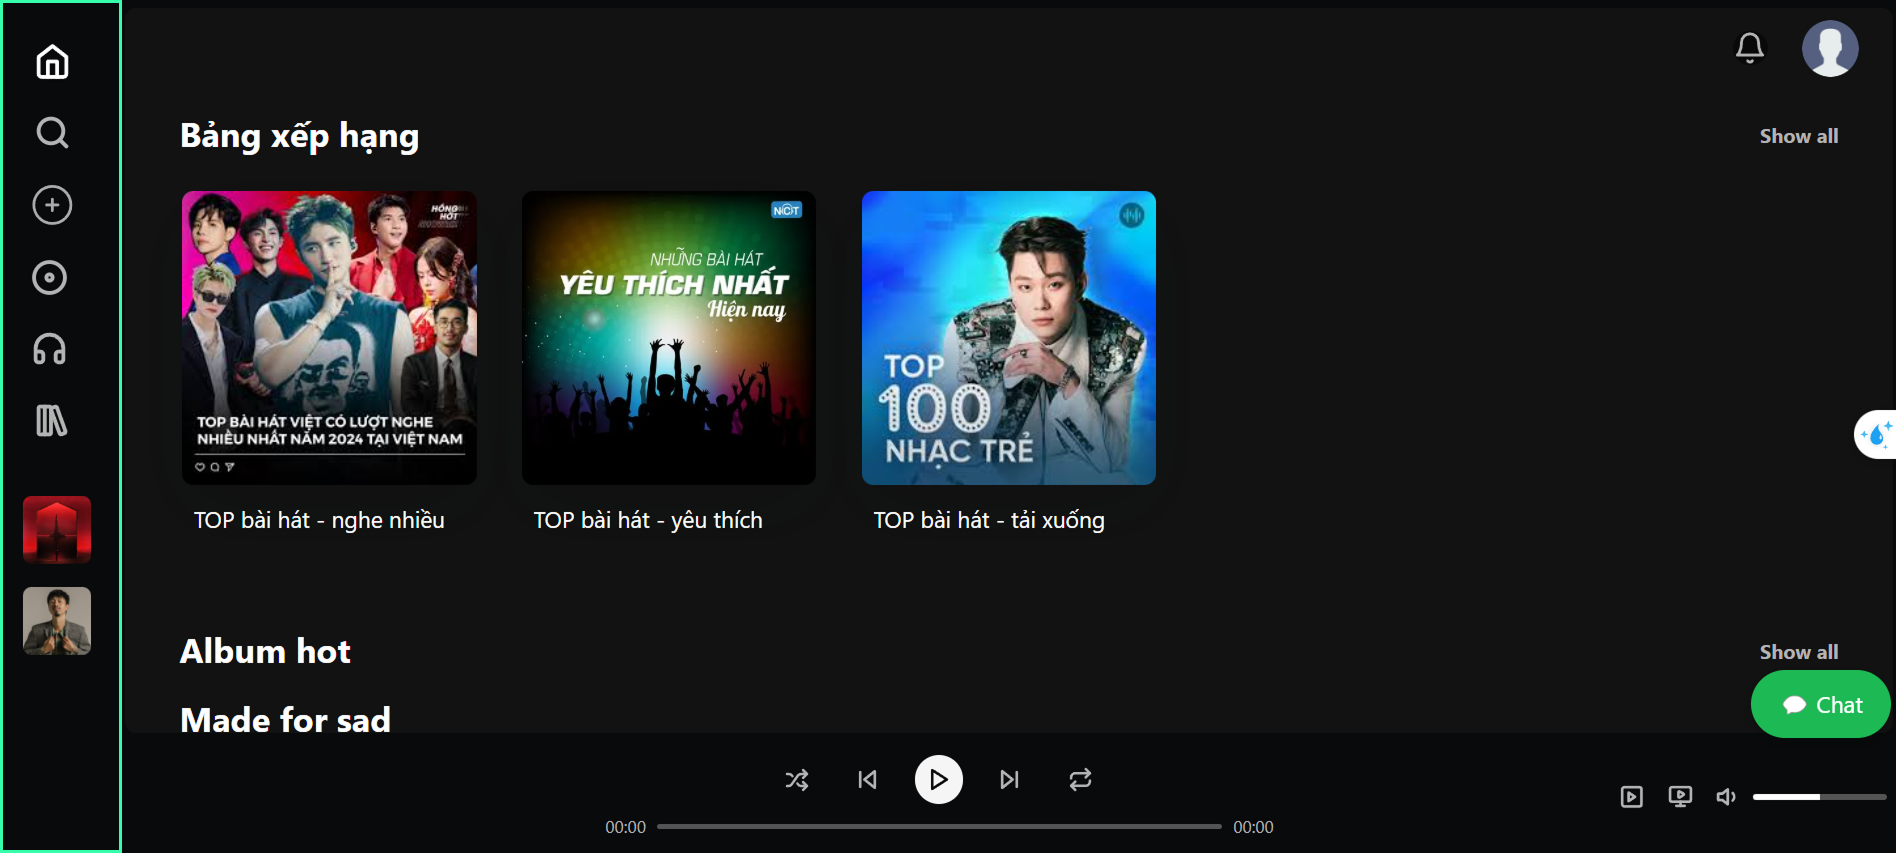
\includegraphics[width=1\textwidth]{imgs/trienkhaife/sidebartop.png}
        \caption{Side Bar Top}
    \end{figure}
  \end{itemize}

  \item \textbf{B. Tạo danh sách phát (playlist):}
  \begin{enumerate}
    \item Nhấn vào biểu tượng \textbf{+} để mở biểu mẫu nhập thông tin playlist.
    \item Nhập các trường: tên, mô tả, ảnh.
    \item Gửi dữ liệu \texttt{FormData} qua API: \texttt{POST /danhsachphat/them/}.
    \item Nếu thành công:
    \begin{itemize}
      \item Reset form, hiển thị thông báo.
      \item Gọi hàm \texttt{refresh()} để cập nhật giao diện.
      \begin{figure}[H]
        \centering
        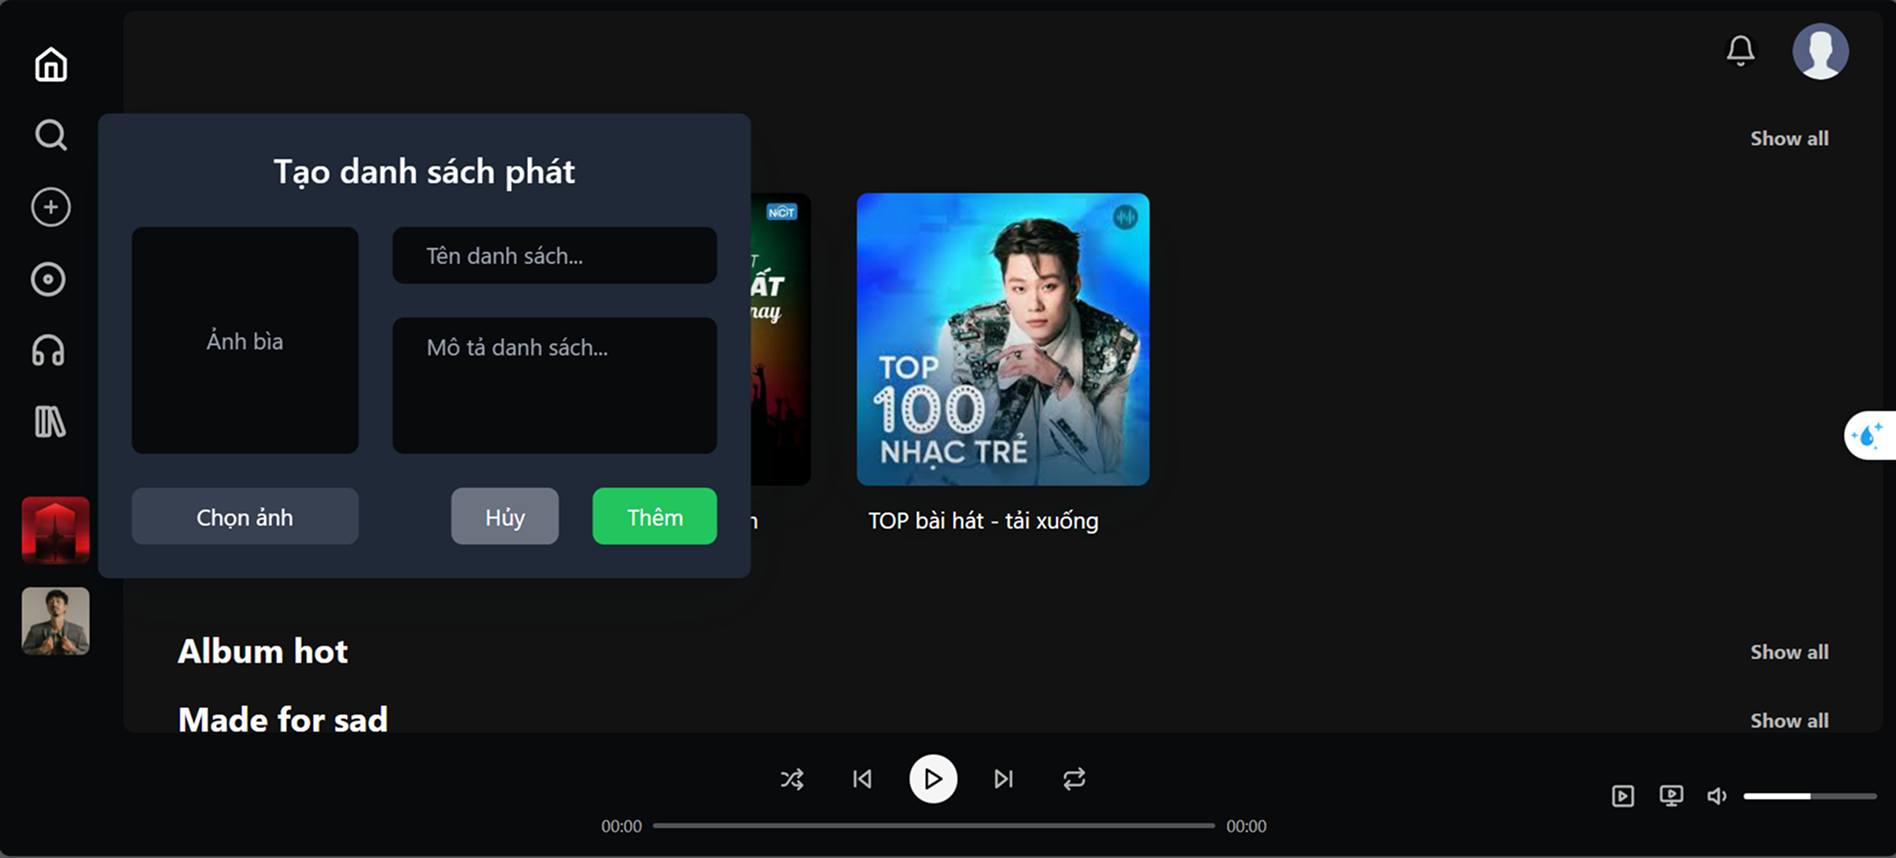
\includegraphics[width=1\textwidth]{imgs/trienkhaife/createPlaylist.png}
        \caption{Tạo Playlist}
      \end{figure}
    \end{itemize}
  \end{enumerate}

  \item \textbf{C. Tạo album:}
  \begin{enumerate}
    \item Nhấn vào biểu tượng \textbf{Disc} để mở form tạo album.
    \item Nhập các trường: tên album, nghệ sĩ, thể loại, ảnh.
    \item Gọi API lấy danh sách thể loại từ \texttt{/loaibaihat/}.
    \item Gửi dữ liệu \texttt{FormData} tới API: \texttt{POST /album/create/}.
    \begin{figure}[H]
        \centering
        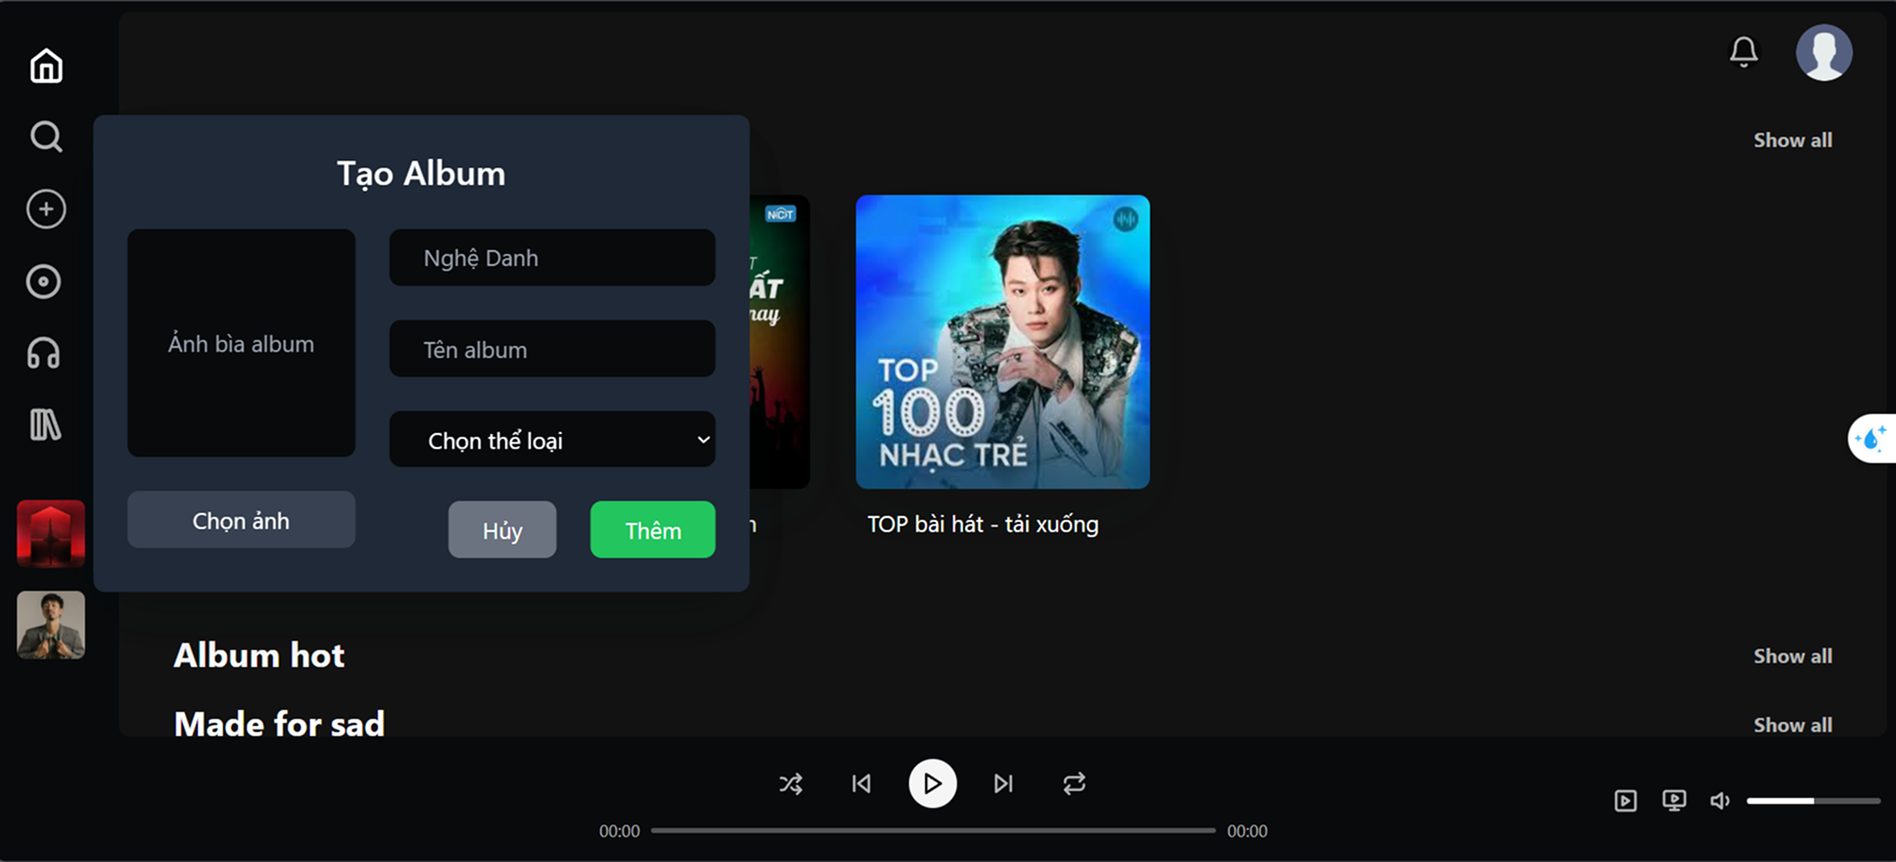
\includegraphics[width=1\textwidth]{imgs/trienkhaife/creatAlbum.png}
        \caption{Tạo Album}
      \end{figure}
  \end{enumerate}

  \item \textbf{D. Tạo playlist theo cảm xúc:}
  \begin{enumerate}
    \item Nhấn vào biểu tượng \textbf{HeadphoneNhấn vào biểu tưs}.
    \item Chọn 1 trong 4 cảm xúc: vui, buồn, thư giãn, sôi động.
    \item Hệ thống chọn ngẫu nhiên một ảnh phù hợp với cảm xúc.
    \item Gửi API: \texttt{POST /danhsachphat/them\_theo\_cam\_xuc/}.
    \begin{figure}[H]
        \centering
        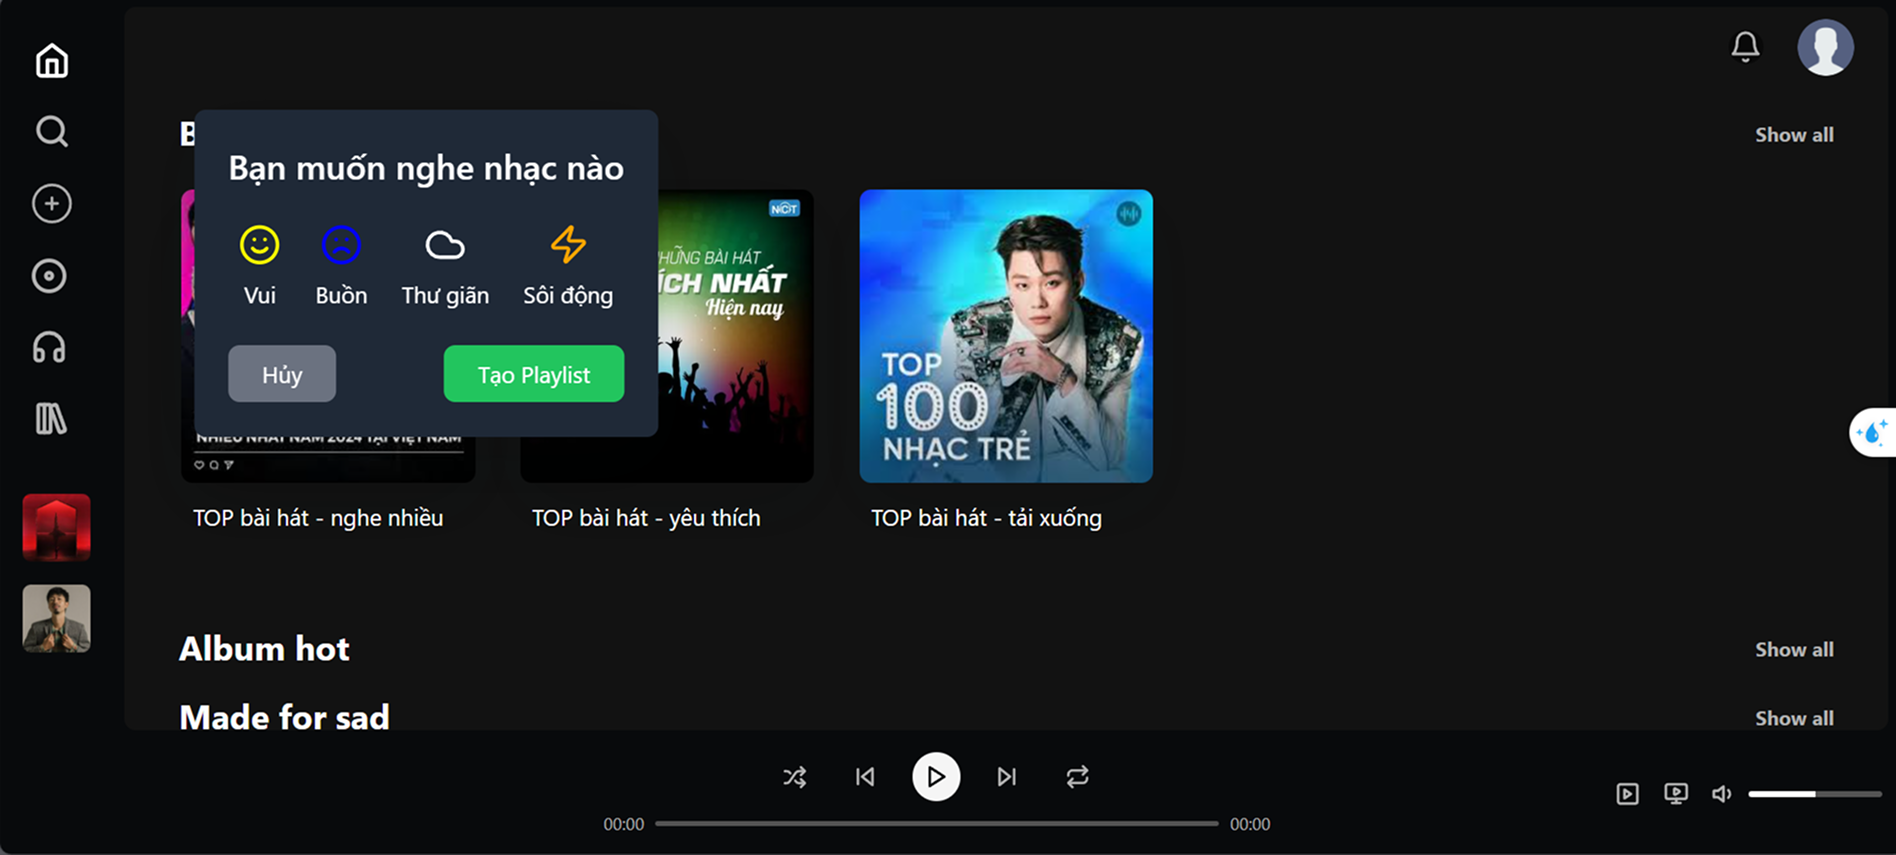
\includegraphics[width=1\textwidth]{imgs/trienkhaife/camxuc.png}
        \caption{Tạo Playlist theo cảm xúc}
      \end{figure}
  \end{enumerate}
  \subsection*{Code minh hoạ các chức năng trong \texttt{SidebarTop}}

\begin{itemize}
  \item \textbf{A. Điều hướng tới các trang chính (Home, Search, Library):}
  \begin{verbatim}
<IconLink Icon={HomeIcon} title="Home" to="/" />
<IconLink Icon={SearchIcon} title="Search" to="/search" />
<TooltipWrapper tooltipContent="Expand Your Library">
  <LibraryBig />
</TooltipWrapper>
  \end{verbatim}

  \item \textbf{B. Tạo danh sách phát mới (Playlist):}
  \begin{itemize}
    \item Hiển thị form nhập tên, mô tả, ảnh:
\begin{verbatim}
{showInput && (
  <form onSubmit={handleSubmit}>
    <input value={playlistName} onChange={...} />
    <textarea value={playlistDescription} />
    <input type="file" onChange={handleImageChange} />
    <button onClick={handleSubmit}>Thêm</button>
  </form>
)}
\end{verbatim}

    \item Gửi API POST \texttt{/danhsachphat/them/}:
\begin{verbatim}
const formData = new FormData();
formData.append("ten_danh_sach", playlistName);
formData.append("mo_ta", playlistDescription);
formData.append("anh_danh_sach", playlistImage);
await axios.post("http://localhost:8000/danhsachphat/them/", formData);
\end{verbatim}
  \end{itemize}

  \item \textbf{C. Tạo album:}
  \begin{itemize}
    \item Hiển thị form nhập tên, nghệ sĩ, thể loại, ảnh:
\begin{verbatim}
{showAlbumInput && (
  <form onSubmit={handleAlbumSubmit}>
    <input value={albumName} onChange={...} />
    <input value={artistName} onChange={...} />
    <select value={albumGenre} onChange={...}>
      <option value="Pop">Pop</option>
    </select>
    <input type="file" onChange={handleAlbumImageChange} />
    <button onClick={handleAlbumSubmit}>Thêm</button>
  </form>
)}
\end{verbatim}

    \item Gửi API POST \texttt{/album/create/}:
\begin{verbatim}
const formData = new FormData();
formData.append("ten_album", albumName);
formData.append("the_loai", albumGenre);
...
await axios.post("http://127.0.0.1:8000/album/create/", formData);
\end{verbatim}
  \end{itemize}

  \item \textbf{D. Tạo playlist theo cảm xúc:}
  \begin{itemize}
    \item Chọn cảm xúc:
\begin{verbatim}
<Smile onClick={() => handleMoodSelect(1)} />
<Frown onClick={() => handleMoodSelect(2)} />
\end{verbatim}

    \item Gửi cảm xúc và ảnh lên API:
\begin{verbatim}
const formData = new FormData();
formData.append("cam_xuc", moodString);
formData.append("anh_danh_sach", file);
await axios.post("http://127.0.0.1:8000/danhsachphat/them_theo_cam_xuc/", formData);
\end{verbatim}
  \end{itemize}
\end{itemize}

\end{itemize}


\section{LibraryCard}

\textbf{Mục đích:} \\
Component \textit{LibraryCard} dùng để hiển thị một danh sách phát (playlist) trong thư viện của người dùng. Người dùng có thể:
\begin{itemize}
  \item Nhấp chuột để điều hướng đến trang chi tiết playlist.
  \item Nhấp chuột phải để hiển thị menu xác nhận xoá playlist.
\end{itemize}

\textbf{Luồng hoạt động:}
\begin{enumerate}
  \item \textbf{Render card:}
  \begin{itemize}
    \item Nếu \texttt{isCollapsed = true}: hiển thị thu gọn chỉ gồm ảnh và tooltip.
    \item Nếu \texttt{isCollapsed = false}: hiển thị đầy đủ tên và mô tả danh sách.
  \end{itemize}

  \item \textbf{Click chuột trái:}
  \begin{itemize}
    \item Sử dụng \texttt{navigate()} để điều hướng đến \texttt{/playlist/?danhsachphatid=...}.
  \end{itemize}

  \item \textbf{Click chuột phải:}
  \begin{itemize}
    \item Hiển thị modal xác nhận xoá playlist.
    \item Gán \texttt{danh\_sach\_phat\_id} vào state \texttt{selectedId}.
  \end{itemize}

  \item \textbf{Nhấn nút "Xoá":}
  \begin{itemize}
    \item Gửi API: \texttt{DELETE /danhsachphat/xoa/\{id\}/}.
    \item Nếu thành công:
    \begin{itemize}
      \item Đóng modal.
      \item Gọi hàm \texttt{refresh()} để cập nhật danh sách playlist.
    \end{itemize}
  \end{itemize}
  \begin{figure}[H]
    \centering
    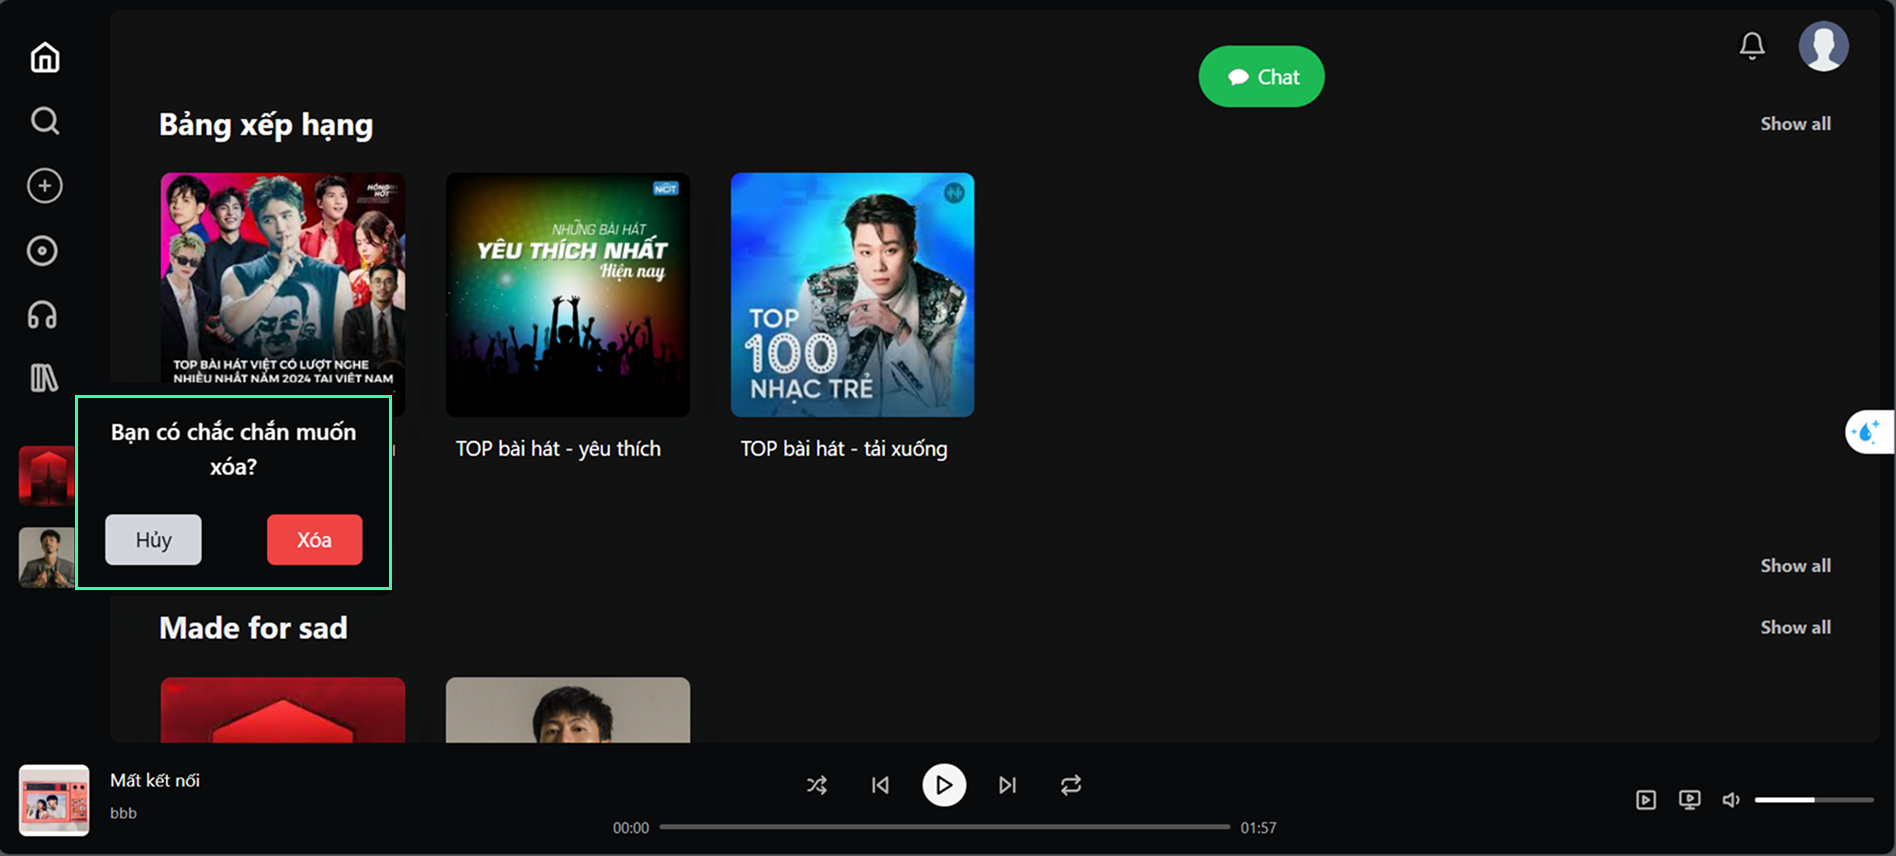
\includegraphics[width=1\textwidth]{imgs/trienkhaife/xoaplaylist.png}
    \caption{Card Library}
  \end{figure}
  \textbf{Code minh hoạ:}

\begin{verbatim}
// A. Điều hướng tới chi tiết playlist
<div onClick={() => navigate(`/playlist/?danhsachphatid=${danh_sach_phat_id}`)}>...</div>

// B. Hiển thị dạng thu gọn (isCollapsed = true)
{isCollapsed && (
  <TooltipWrapper tooltipContent={ten_danh_sach}>
    <div className="p-2 hover:bg-gray-700">
      <LibraryCardImage image={anh_danh_sach} />
    </div>
  </TooltipWrapper>
)}

// C. Hiển thị dạng đầy đủ (isCollapsed = false)
{!isCollapsed && (
  <div className="p-2 hover:bg-gray-700">
    <LibraryCardContent name={ten_danh_sach} songCount={mo_ta} />
  </div>
)}

// D. Click chuột phải để mở modal xoá
<div onContextMenu={handleRightClick}>...</div>

// E. Modal xác nhận xoá
{isModalOpen && (
  <div className="modal">
    <p>Bạn có chắc chắn muốn xoá?</p>
    <button onClick={handleDelete}>Xoá</button>
    <button onClick={() => setIsModalOpen(false)}>Huỷ</button>
  </div>
)}

// F. Gửi API xoá
const handleDelete = async () => {
  await axios.delete(`http://127.0.0.1:8000/danhsachphat/xoa/${selectedId}/`);
  refresh(); // cập nhật danh sách
}
\end{verbatim}
\end{enumerate}


\section{Search}

\textbf{Mục đích:} \\
Trang \textit{Search} cho phép người dùng tìm kiếm các nội dung như:
\begin{itemize}
  \item Bài hát.
  \item Nghệ sĩ.
  \item Album.
  \item Thêm bài hát vào playlist cá nhân.
\end{itemize}

\textbf{Luồng hoạt động:}
\begin{enumerate}
  \item \textbf{Tìm kiếm:}
  \begin{itemize}
    \item Người dùng nhập từ khóa vào ô tìm kiếm.
    \item Khi nhấn "Tìm kiếm", gửi request tới API:
    \texttt{GET /common/api/search?q=\{query\}}.
  \end{itemize}

  \item \textbf{Xử lý kết quả:}
  \begin{itemize}
    \item Kết quả trả về gồm 3 danh sách:
    \begin{itemize}
      \item \texttt{bai\_hat}: danh sách bài hát.
      \item \texttt{nghe\_si}: danh sách nghệ sĩ.
      \item \texttt{albums}: danh sách album.
    \end{itemize}
    \item Hiển thị theo bộ lọc:
    \texttt{Tất cả}, \texttt{Bài hát}, \texttt{Nghệ sĩ}, \texttt{Album}.
  \end{itemize}

  \item \textbf{Phát nhạc:}
  \begin{itemize}
    \item Khi click vào tên bài hát, phát nhạc bằng trình phát audio mặc định.
  \end{itemize}

  \item \textbf{Chuột phải vào bài hát:}
  \begin{itemize}
    \item Hiển thị menu thêm vào playlist.
    \item Chọn playlist → gửi API:
    \texttt{POST /danhsachphat/them-baihat}.
  \end{itemize}

  \item \textbf{Giao diện ghi âm (\texttt{AudioRecorder}):}
  \begin{itemize}
    \item Cho phép ghi âm để tìm kiếm bài hát qua giọng nói
    (chức năng giả định trong phiên bản hiện tại).
  \end{itemize}
  \begin{figure}[H]
    \centering
    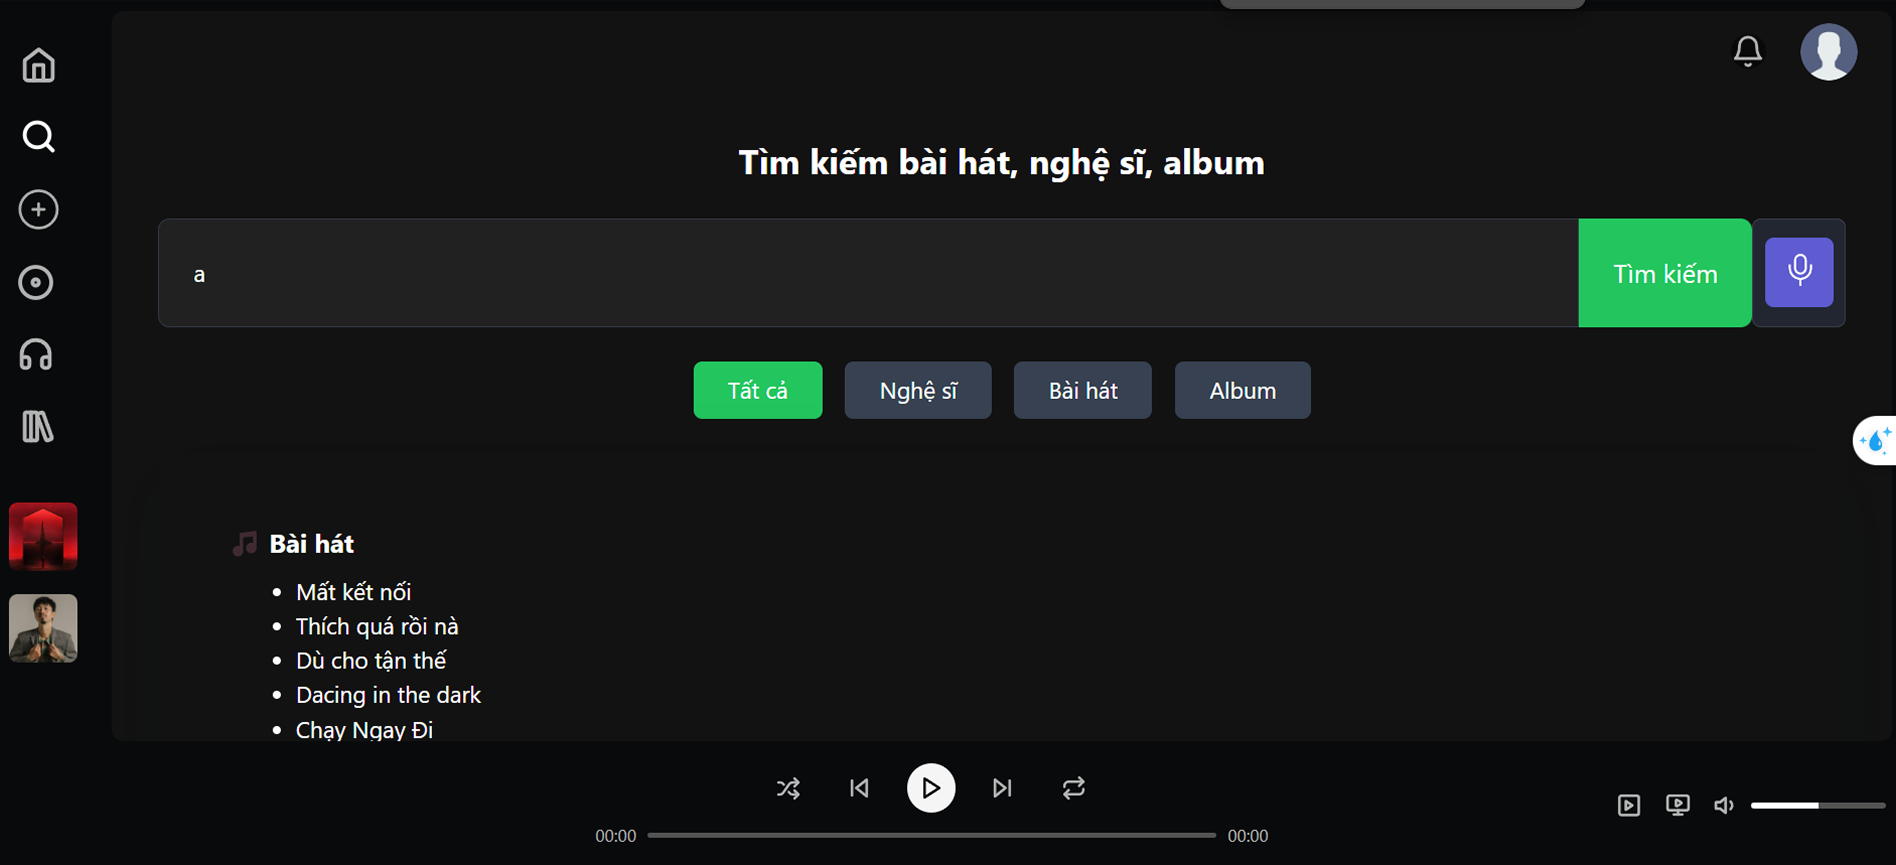
\includegraphics[width=1\textwidth]{imgs/trienkhaife/search.png}
    \caption{Trang tìm kiếm}
  \end{figure}
  \textbf{Code minh hoạ:}

\begin{itemize}
  \item \textbf{A. Người dùng nhập từ khóa và nhấn "Tìm kiếm"}
\begin{verbatim}
<input value={query} onChange={(e) => setQuery(e.target.value)} />
<button onClick={handleSearch}>Tìm kiếm</button>
\end{verbatim}

  \item \textbf{B. Gửi API tìm kiếm GET /common/api/search?q=}
\begin{verbatim}
const handleSearch = async () => {
  const response = await fetch(`http://127.0.0.1:8000/common/api/search?q=${query}`);
  const data = await response.json();
  setResults(data);
};
\end{verbatim}

  \item \textbf{C. Hiển thị danh sách kết quả theo bộ lọc}
\begin{verbatim}
{filter === "bai_hat" && results?.bai_hat.map((song) => (
  <li onClick={() => handleClickSong(song.duong_dan)}>
    {song.ten_bai_hat}
  </li>
))}
\end{verbatim}

  \item \textbf{D. Phát bài hát khi click tên}
\begin{verbatim}
const handleClickSong = (duongDan) => {
  const audio = document.querySelector('#audio-player');
  audio.src = duongDan;
  audio.play();
};
\end{verbatim}

  \item \textbf{E. Chuột phải mở menu "Thêm vào playlist"}
\begin{verbatim}
<li onContextMenu={(e) => handleRightClick(e, song.bai_hat_id)}>
  {song.ten_bai_hat}
</li>
\end{verbatim}

  \item \textbf{F. Hiển thị modal chọn playlist}
\begin{verbatim}
{isModalOpen && (
  <div style={{ top: modalPosition.y, left: modalPosition.x }} className="modal">
    <p>Thêm vào playlist:</p>
    {playlists.map((p) => (
      <div onClick={() => handleAddSongToPlaylist(selectedId, p.danh_sach_phat_id)}>
        {p.ten_danh_sach}
      </div>
    ))}
  </div>
)}
\end{verbatim}

  \item \textbf{G. Gửi API POST /danhsachphat/them-baihat/}
\begin{verbatim}
const handleAddSongToPlaylist = async (bai_hat_id, danh_sach_phat_id) => {
  await fetch("http://127.0.0.1:8000/thembaihatvaodanhsachphat/danhsachphat/them-baihat/", {
    method: "POST",
    headers: { "Content-Type": "application/json" },
    body: JSON.stringify({ bai_hat_id, danh_sach_phat_id }),
  });
};
\end{verbatim}
\end{itemize}
\end{enumerate}


\section{DynamicGrid}

\textbf{Mục đích:} \\
Component \textit{DynamicGrid} hiển thị danh sách các phần tử như \texttt{ItemCard} theo dạng lưới (grid), với số lượng cột tự động theo chiều rộng.

\textbf{Luồng hoạt động:}
\begin{enumerate}
  \item \textbf{Nhận props:}
  \begin{itemize}
    \item \texttt{title, description}: tiêu đề và mô tả.
    \item \texttt{items}: danh sách các đối tượng có \texttt{order}, \texttt{danh\_sach\_phat\_id}.
    \item \texttt{to}: URL đích khi click tiêu đề.
    \item \texttt{Component}: thành phần con để render trong grid.
  \end{itemize}

  \item \textbf{Tính số cột:}
  \begin{itemize}
    \item Dựa vào chiều rộng cửa sổ (\texttt{mainWidth}) chia cho \texttt{cardSizePx = 220} để tính \texttt{columnCount}.
  \end{itemize}

  \item \textbf{Render:}
  \begin{itemize}
    \item Hiển thị tiêu đề + nút ``Show all''.
    \item Render các phần tử đầu tiên (theo số cột), sắp xếp theo \texttt{order}.
  \end{itemize}

  \item \textbf{Click ``Show all'':}
  \begin{itemize}
    \item Điều hướng tới \texttt{/showall} và truyền \texttt{items} qua \texttt{state}.
  \end{itemize}
  \begin{figure}[H]
    \centering
    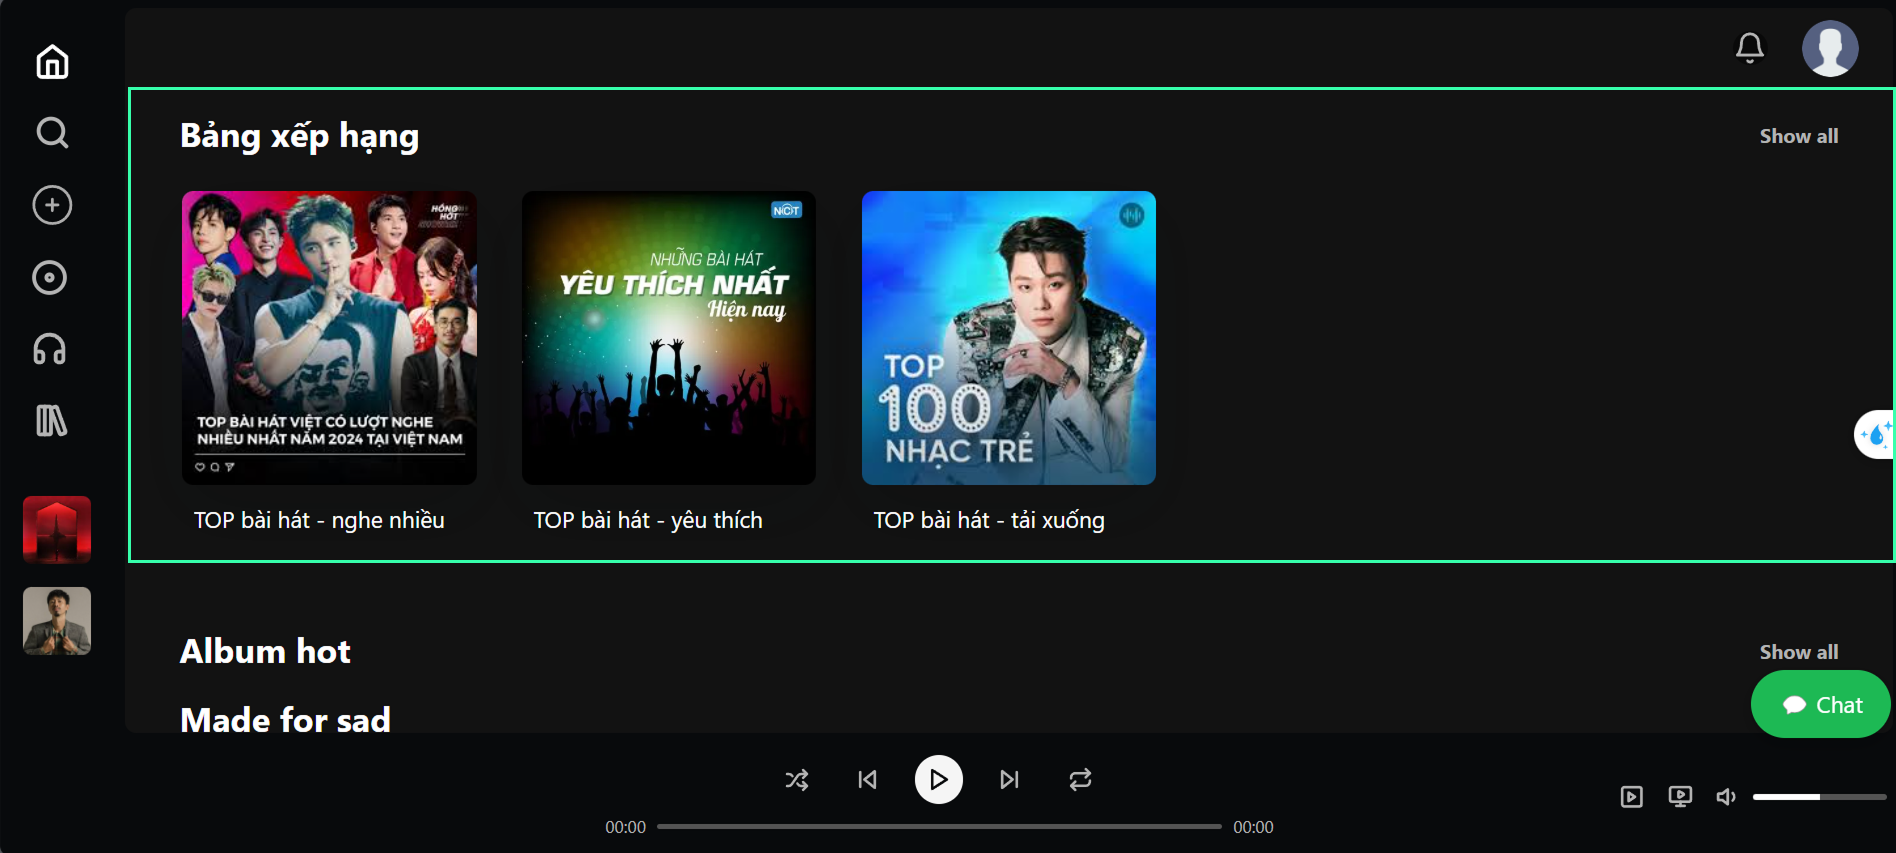
\includegraphics[width=1\textwidth]{imgs/trienkhaife/dynamic.png}
    \caption{DynamicGrid}
  \end{figure}
  \textbf{Code minh họa}

\begin{verbatim}
// A. Nhận props: title, description, items, to, Component
function DynamicGrid({ title, description, items, to, Component }) {
  const width = useAppControllerStore((state) => state.mainWidth);
  const columnCount = Math.floor(width / 220); // B. Tính số cột

  return (
    <div>
      // C. Header hiển thị tiêu đề và nút Show all
      <div className="flex justify-between items-center px-3.5 py-2">
        <Link to={to || '/'}>
          <h2 className="text-white text-2xl font-bold hover:underline">{title}</h2>
        </Link>
        <Link to="/showall" state={{ items }}>
          <span className="text-sm text-gray-400 hover:underline">Show all</span>
        </Link>
      </div>

      // D. Hiển thị mô tả nếu có
      {description && <p className="px-3.5 text-sm text-gray-400">{description}</p>}

      // E. Hiển thị grid các item
      <div
        style={{ display: 'grid', gridTemplateColumns: `repeat(${columnCount}, minmax(0, 1fr))` }}
        className="gap-4 px-3.5 mt-4"
      >
        {items
          .slice(0, columnCount)
          .sort((a, b) => a.order - b.order)
          .map((item) => (
            <Component key={item.danh_sach_phat_id} {...item} />
          ))}
      </div>
    </div>
  );
}
\end{verbatim}

\end{enumerate}

\section{ItemCard}

\textbf{Mục đích:} \\
Hiển thị một thẻ danh sách nhạc (playlist, album, hoặc bảng xếp hạng), cho phép điều hướng đến chi tiết tương ứng.

\textbf{Luồng hoạt động:}
\begin{enumerate}
  \item Nhận props: \texttt{danh\_sach\_phat\_id}, \texttt{album\_id}, \texttt{bxh\_id}, ảnh, tên, mô tả.
  \item Render:
  \begin{itemize}
    \item Hiển thị ảnh, tên danh sách (rút gọn nếu dài).
    \item Hiển thị mô tả nếu có.
  \end{itemize}
  \item Khi click vào thẻ:
  \begin{itemize}
    \item Dùng \texttt{useNavigate()} điều hướng đến \texttt{/playlist/?...} tùy loại dữ liệu.
  \end{itemize}
  \begin{figure}[H]
    \centering
    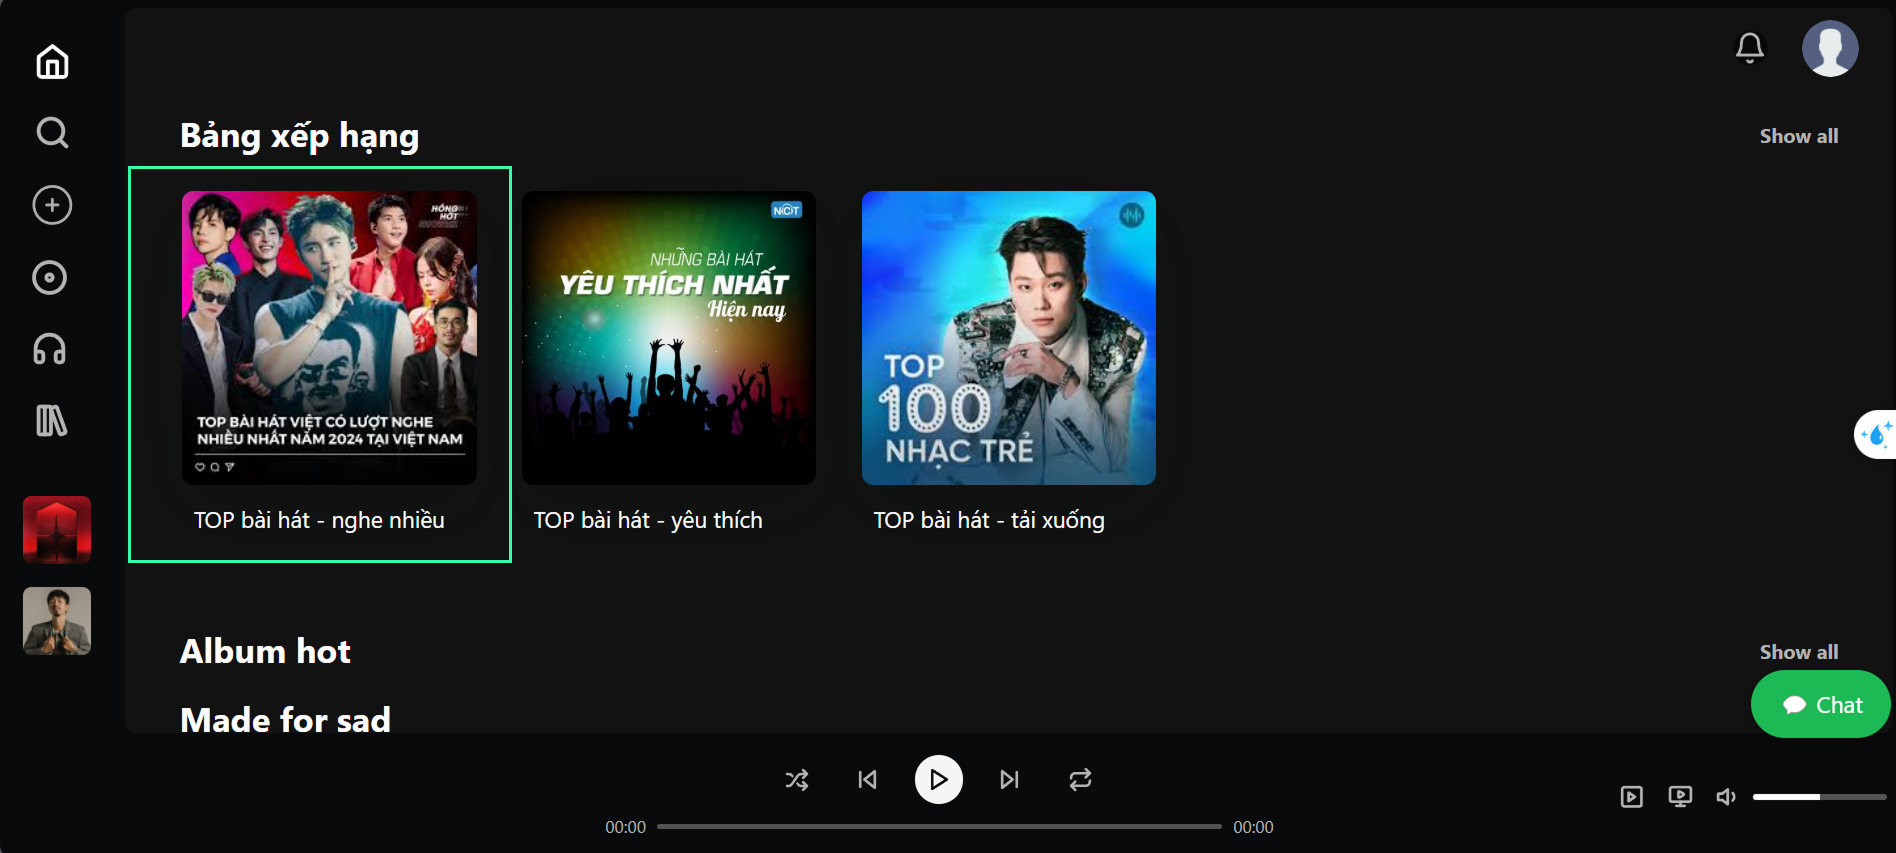
\includegraphics[width=1\textwidth]{imgs/trienkhaife/itemcard.png}
    \caption{ItemCard}
  \end{figure}
  \textbf{Code minh họa:}

\begin{verbatim}
// A. Nhận props từ cha: ID, ảnh, tên, mô tả
function ItemCard({ danh_sach_phat_id, album_id, bxh_id, anh_danh_sach, ten_danh_sach, description }) {
  const navigate = useNavigate();

  // B. Xác định đường dẫn cần điều hướng
  const openSong = () => {
    if (danh_sach_phat_id) navigate(`/playlist/?danhsachphatid=${danh_sach_phat_id}`);
    else if (album_id) navigate(`/playlist/?albumid=${album_id}`);
    else if (bxh_id) navigate(`/playlist/?bxh=${bxh_id}`);
  };

  return (
    // C. Click vào thẻ để điều hướng
    <div onClick={openSong} className="group relative flex flex-col p-3 hover:bg-white/10 cursor-pointer">

      {/* D. Hiển thị ảnh */}
      <img src={anh_danh_sach} className="w-full aspect-square object-cover rounded-lg shadow-lg" />

      {/* E. Tên danh sách (giới hạn chiều dài) */}
      <p className="truncate text-white pt-3">{ten_danh_sach}</p>

      {/* F. Mô tả nếu có, nếu không để trống */}
      {description ? (
        <p className="text-sm text-gray-400 line-clamp-2">{description}</p>
      ) : (
        <div className="h-5"></div>
      )}
    </div>
  );
}
\end{verbatim}

\end{enumerate}

\section{PlaylistDetail}

\textbf{Mục đích:} \\
Trang chi tiết cho playlist, album hoặc BXH, hỗ trợ phát nhạc, thêm bài hát, và hiển thị thông tin.

\textbf{Luồng xử lý:}
\begin{enumerate}
  \item \textbf{Xác định loại dữ liệu:}
  \begin{itemize}
    \item Dựa vào URL: \texttt{?danhsachphatid}, \texttt{?albumid}, \texttt{?bxh}.
    \item Gọi API tương ứng: \texttt{/danhsachphat/}, \texttt{/album/}, \texttt{/bxh/}.
  \end{itemize}

  \item \textbf{Lấy danh sách bài hát:}
  \begin{itemize}
    \item Gọi \texttt{getSongById()}, lấy nghệ sĩ và album.
    \item Nếu không Premium:
    \begin{itemize}
      \item Chèn quảng cáo mỗi 2 bài.
      \item Bài Premium sẽ phát audio thay thế.
    \end{itemize}
  \end{itemize}

  \item \textbf{Phát nhạc:}
  \begin{itemize}
    \item Click 1 lần chọn bài, click 2 lần phát.
    \item Nếu không Premium và đã nghe quá 2 bài, phát quảng cáo 30s.
  \end{itemize}

  \item \textbf{Giao diện bài hát:}
  \begin{itemize}
    \item Hiển thị STT | Tên | Album | Ngày phát hành | Thời lượng | Lượt nghe.
    \item Cho phép thêm vào playlist khác bằng chuột phải.
  \end{itemize}

  \item \textbf{Thêm bài hát (nếu album chờ duyệt):}
  \begin{itemize}
    \item Hiển thị modal nhập thông tin + upload file nhạc.
    \item Gửi lên API dạng \texttt{FormData} qua \texttt{addBaiHat}.
  \end{itemize}
  \begin{figure}[H]
    \centering
    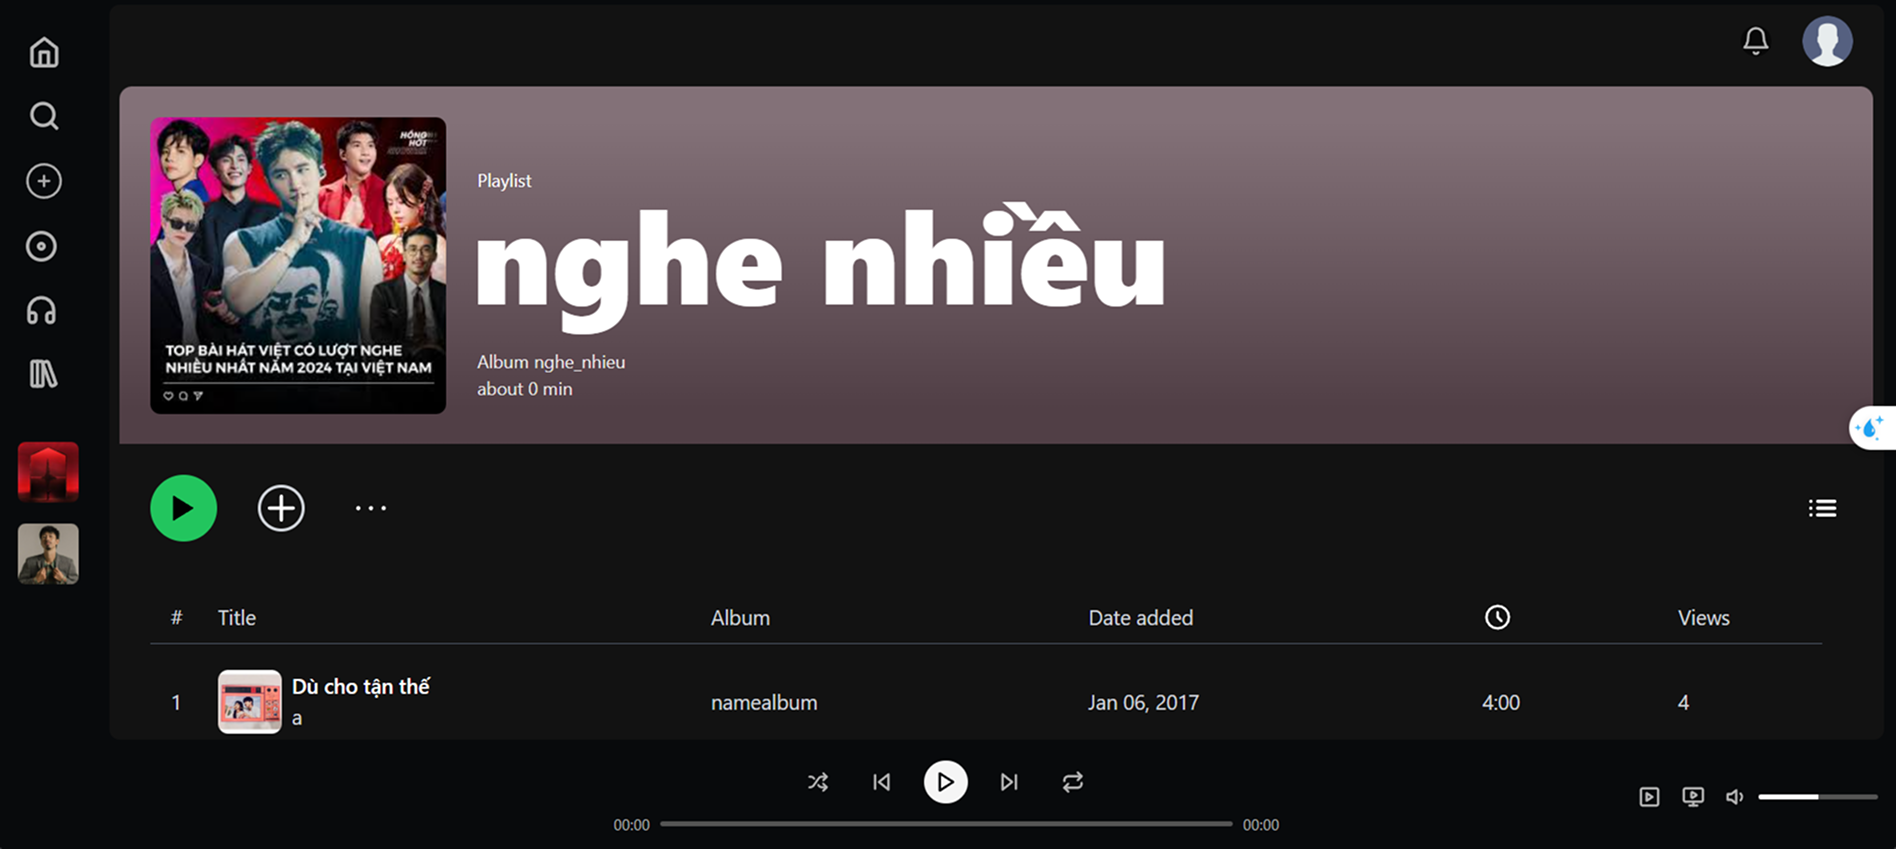
\includegraphics[width=1\textwidth]{imgs/trienkhaife/playlist.png}
    \caption{Trang Playlist}
  \end{figure}
  \subsection*{Code minh hoạ luồng xử lý phát Playlist}

\begin{itemize}
  \item \textbf{A. Xác định loại playlist từ URL:}
\begin{verbatim}
const searchParams = new URLSearchParams(location.search);
const danhSachPhatId = searchParams.get('danhsachphatid');
const albumId = searchParams.get('albumid');
const bxh = searchParams.get('bxh');
const playlistId = danhSachPhatId || albumId || bxh;
\end{verbatim}

  \item \textbf{B. Gọi API lấy danh sách bài hát:}
\begin{verbatim}
useEffect(() => {
  async function fetchSongs() {
    let rawSongs;
    if (danhSachPhatId) rawSongs = await getSongFromPlayList(playlistId);
    else if (albumId) rawSongs = await getSongAlbum(playlistId);
    else rawSongs = await getSongBXH(playlistId);

    const details = await Promise.all(rawSongs.map(async ({ bai_hat }) => {
      const song = await getSongById(bai_hat);
      return {
        ...song,
        nghe_si: (await axios.get(`/api/nghesi/${song.nghe_si}`)).data.ten_nghe_si,
        ten_album: (await axios.get(`/album/${song.album}`)).data.ten_album,
      };
    }));

    const isPremium = (await getUserInfo("")).la_premium;
    const finalSongs = [];
    details.forEach((s, i) => {
      if (!isPremium && s.is_premium) s.duong_dan = '/ad.mp3';
      finalSongs.push(s);
      if ((i + 1) % 2 === 0 && !isPremium)
        finalSongs.push({ the_loai: 'Ad', ten_bai_hat: 'Quảng cáo', duong_dan: '/ad.mp3' });
    });
    setSongs(finalSongs);
  }
  fetchSongs();
}, [playlistId]);
\end{verbatim}

  \item \textbf{C. Phát bài hát khi người dùng click 2 lần:}
\begin{verbatim}
const handleClick = (song) => {
  if (!isPremium && songsPlayed >= 2) return playAdThen(song);
  dispatch(setCurrentSong(song));
  playAudio(song.duong_dan);
};
\end{verbatim}


  \item \textbf{D. Hiển thị danh sách bài hát:}
\begin{verbatim}
songs.map((s, i) => (
  <div key={i} onClick={() => handleClick(s)}>
    {i+1}. {s.ten_bai_hat} - {s.nghe_si} ({s.ten_album})
  </div>
));
\end{verbatim}

  \item \textbf{E. Nếu là nghệ sĩ và album đang pending, cho phép thêm bài hát:}
\begin{verbatim}
if (albumPending) {
  <Button onClick={() => setShowModal(true)}>Thêm bài hát</Button>
}
\end{verbatim}
\end{itemize}

\end{enumerate}

\section{TrackDetail}

\textbf{Mục đích:} \\
Hiển thị chi tiết một bài hát, gồm phát nhạc, lời bài hát (đồng bộ thời gian), và thông tin liên quan.

\textbf{Luồng xử lý:}
\begin{enumerate}
  \item Lấy \texttt{id} từ URL \texttt{/track/:id} và gọi \texttt{getSongById()}.
  \item Gọi API lấy album và nghệ sĩ tương ứng.
  \item Phát nhạc: set \texttt{audioPlayer.src}, gọi \texttt{play()}, dispatch \texttt{setCurrentSong(song)}.
  \item Lời bài hát:
  \begin{itemize}
    \item Phân tích \texttt{loi\_bai\_hat} theo timestamp \texttt{[hh:mm:ss]}.
    \item Đồng bộ với \texttt{audio.currentTime}, làm nổi bật dòng đang phát.
  \end{itemize}
  \item Phân tích ảnh bìa tạo màu nền gradient tương ứng.
  \begin{figure}[H]
    \centering
    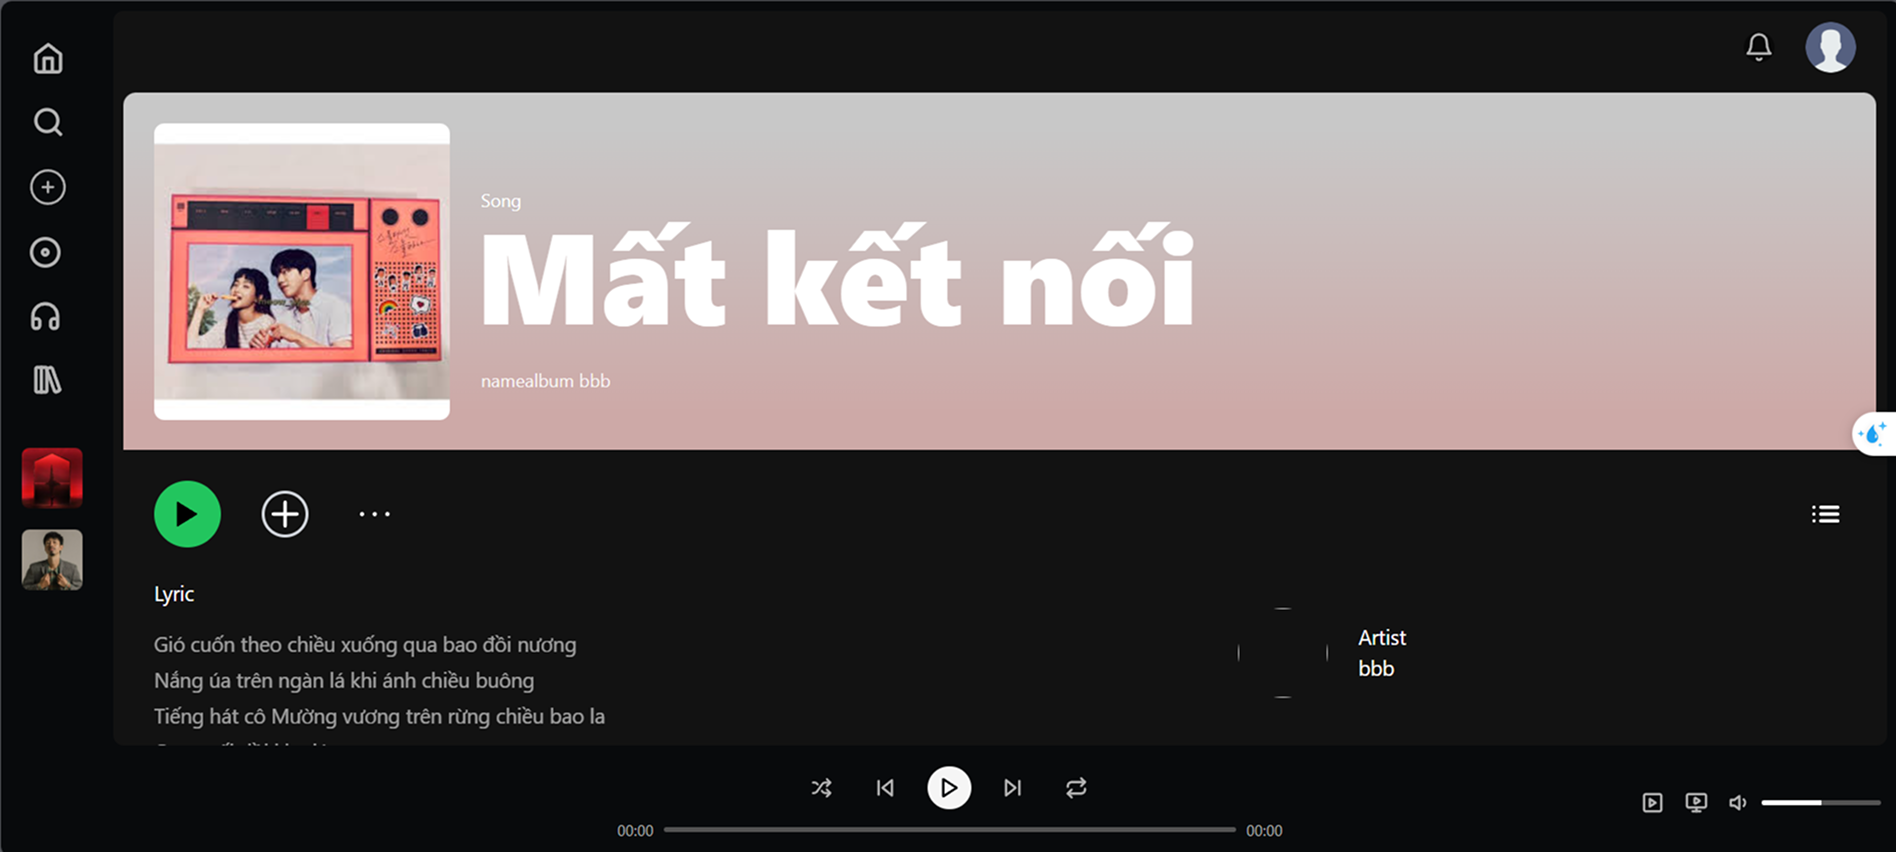
\includegraphics[width=1\textwidth]{imgs/trienkhaife/track.png}
    \caption{Trang Track}
  \end{figure}
\end{enumerate}

\section{VideoPlayer}

\textbf{Mục đích:} \\
Hiển thị và đồng bộ video bài hát đang phát, hỗ trợ tải về nếu có video.

\textbf{Luồng xử lý:}
\begin{enumerate}
  \item Lấy bài hát hiện tại từ Redux: \texttt{state.player.currentSong}.
  \item Phân biệt video hay mp3:
  \begin{itemize}
    \item Nếu \texttt{.mp3} thì không có video.
    \item Nếu là video (\texttt{.mp4}, ...) thì hiển thị thẻ \texttt{<video>}.
  \end{itemize}
  \item Đồng bộ thời gian: mỗi 500ms cập nhật \texttt{video.currentTime = audio.currentTime}.
  \item Khi isPaused thay đổi: \texttt{pause/play} video.
  \item Tải video/audio: fetch \texttt{videoUrl}, gọi \texttt{saveAs()} với tên bài hát.
  \begin{figure}[H]
    \centering
    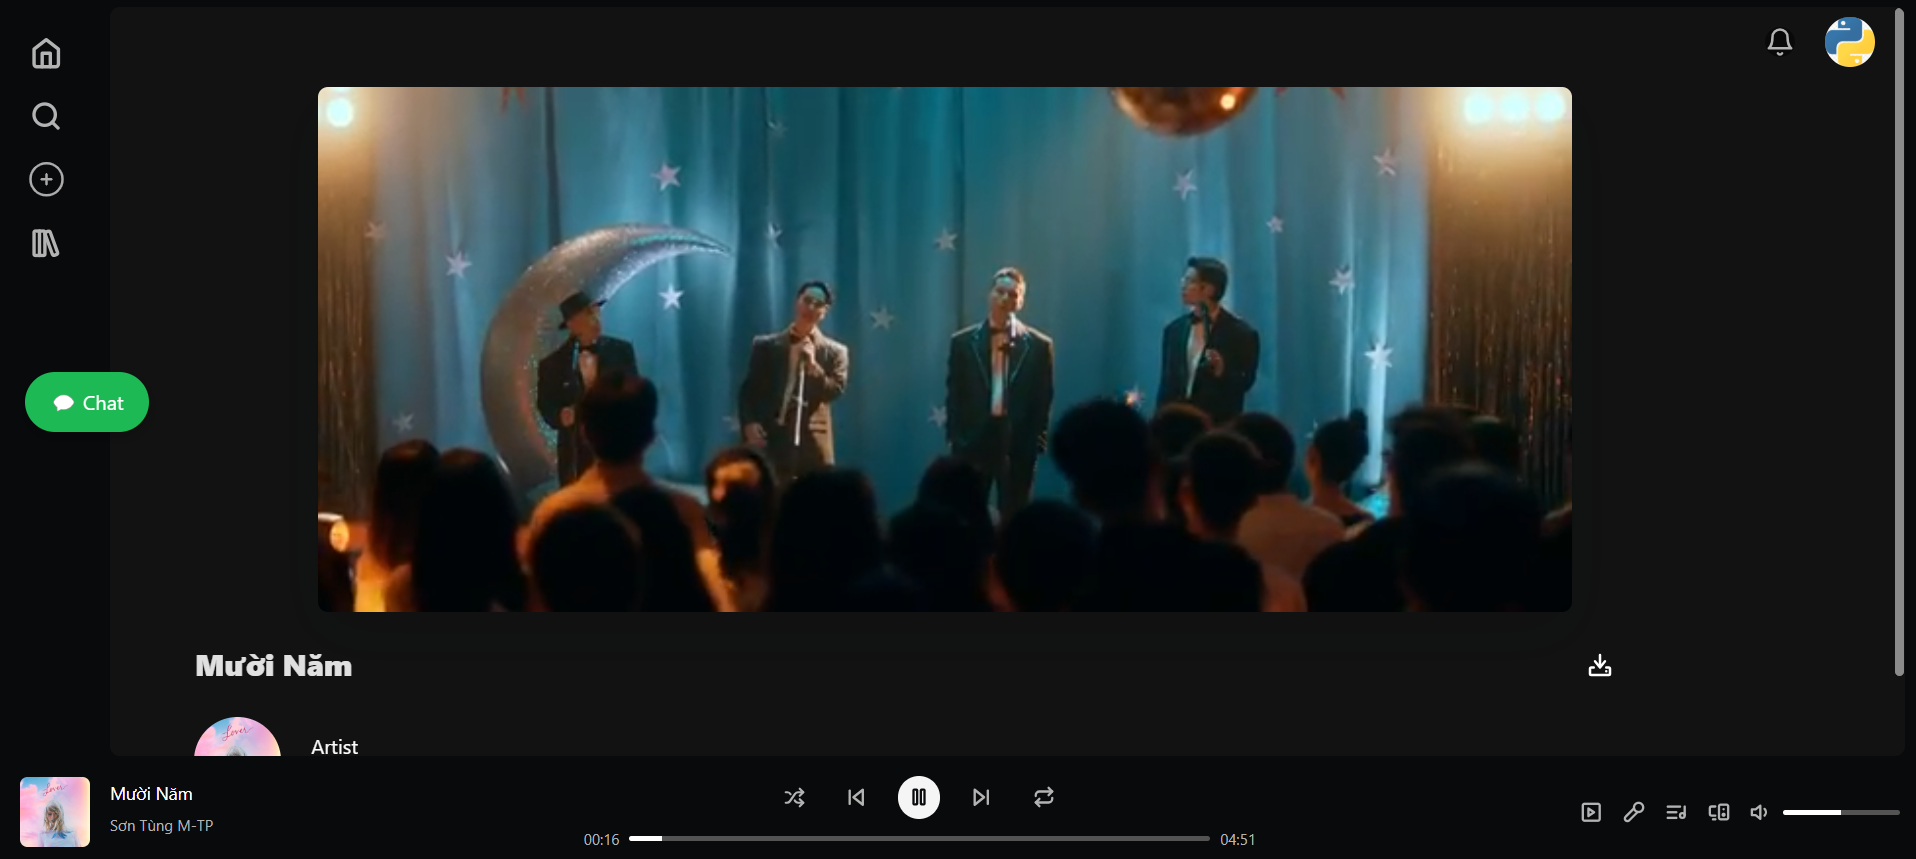
\includegraphics[width=1\textwidth]{imgs/chap5/phat_video.png}
    \caption{Trang xem video}
  \end{figure}

  \subsection*{Code minh hoạ luồng xử lý phát Video/Audio}

\begin{itemize}
  \item \textbf{A. Lấy bài hát hiện tại và kiểm tra có video không:}
\begin{verbatim}
const currentSong = useSelector((state) => state.player.currentSong);
const isVideo = currentSong?.duong_dan?.endsWith('.mp4') || 
                currentSong?.duong_dan?.endsWith('.webm');
\end{verbatim}

  \item \textbf{B. Đồng bộ thời gian video = audio mỗi 500ms:}
\begin{verbatim}
useEffect(() => {
  const audio = document.querySelector('#audio-player');
  const sync = () => videoRef.current && audio && 
                  (videoRef.current.currentTime = audio.currentTime);
  const interval = setInterval(sync, 500);
  return () => clearInterval(interval);
}, []);
\end{verbatim}

  \item \textbf{C. Khi tab bị ẩn rồi hiện lại, video phát từ vị trí cũ:}
\begin{verbatim}
useEffect(() => {
  const resume = () => !document.hidden && videoRef.current?.play();
  document.addEventListener('visibilitychange', resume);
  return () => document.removeEventListener('visibilitychange', resume);
}, []);
\end{verbatim}

  \item \textbf{D. Đồng bộ trạng thái Play/Pause với video:}
\begin{verbatim}
useEffect(() => {
  if (videoRef.current) {
    isPaused ? videoRef.current.pause() : videoRef.current.play();
  }
}, [isPaused]);
\end{verbatim}

  \item \textbf{E. Nút tải xuống video/audio khi người dùng bấm:}
\begin{verbatim}
const download = async () => {
  const res = await fetch(currentSong.duong_dan);
  const blob = await res.blob();
  saveAs(blob, `${currentSong.ten_bai_hat}.mp4`);
};
\end{verbatim}

  \item \textbf{F. Hiển thị giao diện:}
\begin{verbatim}
return (
  <div>
    {isVideo ? (
      <video ref={videoRef} src={currentSong.duong_dan} autoPlay muted />
    ) : (
      <p>Bài hát này không có video</p>
    )}
    {isVideo && <button onClick={download}>Tải xuống</button>}
  </div>
);
\end{verbatim}
\end{itemize}

\end{enumerate}


\section{TrackDisplayer}
\textbf{Mục đích:} TrackDisplayer là component nhỏ hiển thị thông tin bài hát đang phát tại thanh điều khiển, gồm:
\begin{itemize}
  \item Ảnh bìa album.
  \item Tên bài hát.
  \item Tên nghệ sĩ.
\end{itemize}

\textbf{Luồng xử lý:}
\begin{enumerate}
  \item Nhận các props đầu vào:
  \begin{itemize}
    \item \texttt{song}: thông tin bài hát hiện tại.
    \item \texttt{artist}: đối tượng nghệ sĩ (nếu cần chi tiết).
    \item \texttt{artistName}: tên nghệ sĩ dạng chuỗi.
  \end{itemize}
  \item Gọi API lấy thông tin album:
  \begin{itemize}
    \item Dùng \texttt{song.album\_id} để gửi GET tới \texttt{/album/:id}.
    \item Lưu kết quả vào state \texttt{album}.
  \end{itemize}
  \item Render giao diện:
  \begin{itemize}
    \item Nếu có dữ liệu: hiển thị ảnh bìa, tên bài hát và tên nghệ sĩ.
  \end{itemize}
  \begin{figure}[H]
    \centering
    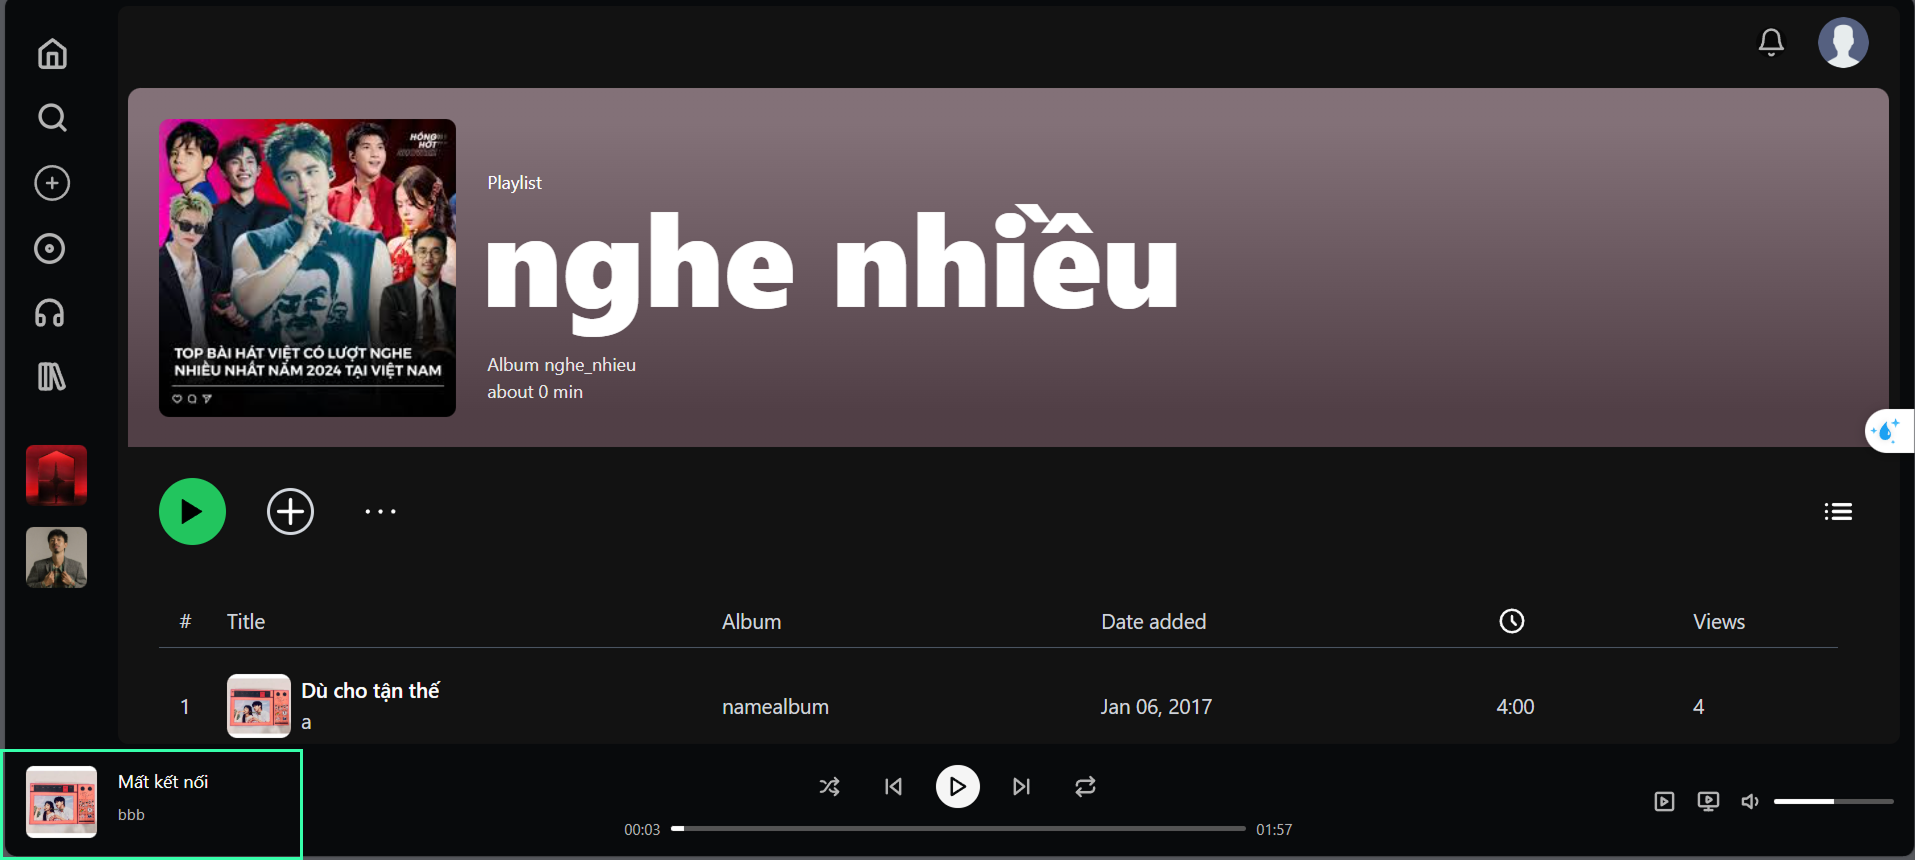
\includegraphics[width=1\textwidth]{imgs/trienkhaife/trackdisplay.png}
    \caption{Bài hát đang phát}
  \end{figure}
  \subsection*{Code minh hoạ hiển thị thông tin bài hát hiện tại}

  \textbf{A. Nhận props đầu vào:}
  \begin{verbatim}
  type Props = {
    song: { album_id: number; ten_bai_hat: string } | null;
    artistName: string;
  };
  \end{verbatim}
  
  \textbf{B. Gọi API lấy thông tin album:}
  \begin{verbatim}
  useEffect(() => {
    if (!song?.album_id) return;
    axios.get(`http://127.0.0.1:8000/album/${song.album_id}/`)
      .then(res => setAlbum(res.data))
      .catch(err => console.error("Lỗi lấy album:", err));
  }, [song]);
  \end{verbatim}
  
  \textbf{C. Render thông tin bài hát:}
  \begin{verbatim}
  if (!song || !album) return null;
  
  return (
    <div className="flex items-center gap-3">
      <img src={album.anh_bia} alt="cover" className="w-14 h-14 rounded-md" />
      <div>
        <div className="text-white text-sm">{song.ten_bai_hat}</div>
        <div className="text-gray-400 text-xs">{artistName}</div>
      </div>
    </div>
  );
  \end{verbatim}
\end{enumerate}

\section{ButtonGroup}
\textbf{Mục đích:} ButtonGroup là nhóm các nút điều khiển nhạc trung tâm, bao gồm:
\begin{itemize}
  \item Play / Pause
  \item Next / Previous
  \item Shuffle (ngẫu nhiên)
  \item Repeat (lặp một bài / toàn danh sách)
\end{itemize}

\textbf{Luồng xử lý:}
\begin{enumerate}
  \item \textbf{Play/Pause:}
  \begin{itemize}
    \item Kiểm tra trạng thái \texttt{isPaused} từ Redux.
    \item Nếu đang pause → gọi \texttt{audio.play()} và cập nhật Redux.
    \item Nếu đang phát → gọi \texttt{audio.pause()} và cập nhật Redux.
  \end{itemize}

  \item \textbf{Next / Previous:}
  \begin{itemize}
    \item Nếu bài hiện tại là quảng cáo (the\_loai = "Advertisement") → chặn next/prev.
    \item Nếu bật \texttt{Shuffle}:
    \begin{itemize}
      \item Phát bài tiếp theo trong danh sách đã được xáo trộn (\texttt{shuffledList}).
    \end{itemize}
    \item Nếu không Shuffle:
    \begin{itemize}
      \item Xác định bài tiếp theo dựa vào chỉ số hiện tại \texttt{currentIndex}.
    \end{itemize}
  \end{itemize}

  \item \textbf{Repeat:}
  \begin{itemize}
    \item Có 3 chế độ: \texttt{none}, \texttt{one}, \texttt{all}.
    \item Tùy vào trạng thái, sự kiện \texttt{audio.onended} sẽ có hành vi:
    \begin{itemize}
      \item \texttt{one}: phát lại bài hiện tại.
      \item \texttt{all}: phát bài tiếp theo, nếu hết thì quay lại đầu danh sách.
      \item \texttt{none}: dừng lại khi kết thúc danh sách.
    \end{itemize}
  \end{itemize}

  \item \textbf{Shuffle:}
  \begin{itemize}
    \item Khi bật:
    \begin{itemize}
      \item Tạo danh sách mới đã được xáo trộn bằng \texttt{shuffleArray}.
      \item Gán \texttt{idShuffledList} cho mỗi bài để theo dõi.
    \end{itemize}
    \item Khi tắt:
    \begin{itemize}
      \item Trở lại danh sách gốc \texttt{listAudio}.
    \end{itemize}
  \end{itemize}
  \begin{figure}[H]
    \centering
    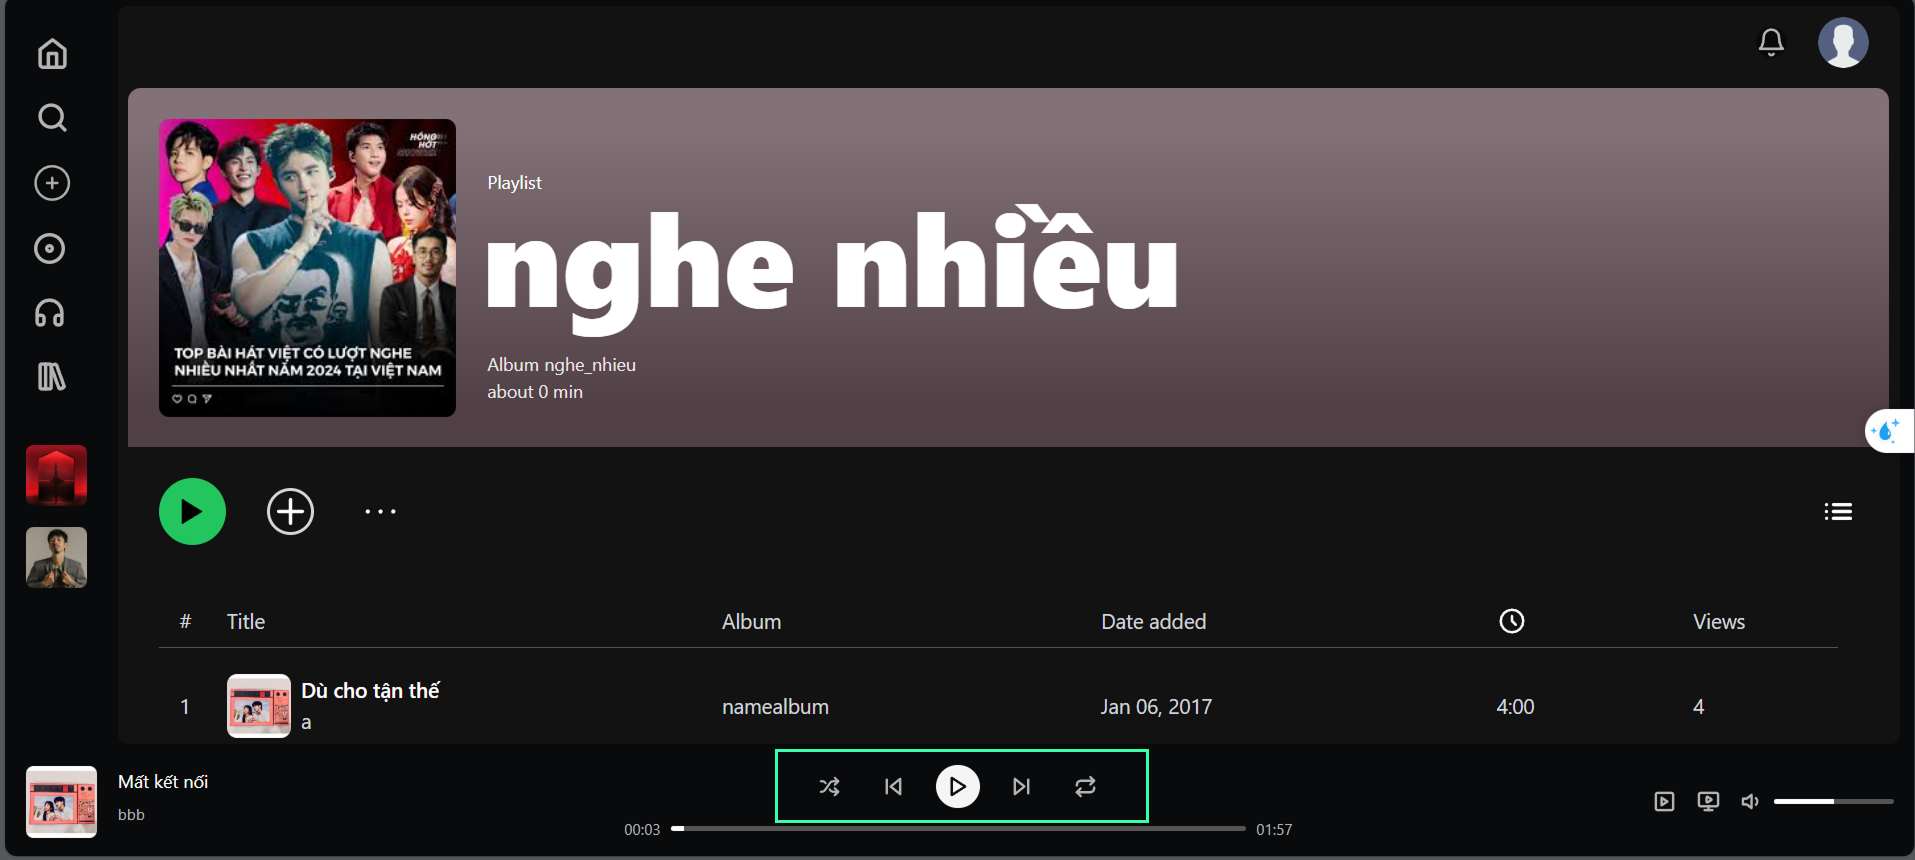
\includegraphics[width=1\textwidth]{imgs/trienkhaife/btn-group.png} 
    \caption{Các nút điều khiển}
  \end{figure}
  \subsection*{Code minh hoạ ButtonGroup - Điều khiển nhạc}
  \begin{itemize}
    \item \textbf{A. Play/Pause:}
    \begin{verbatim}
  const onPlay = () => {
    isPaused ? audio.play() : audio.pause();
    dispatch(togglePlayPause());
  };
    \end{verbatim}
  
    \item \textbf{B. Next / Previous:}
    \begin{verbatim}
  const play = (i) => {
    const song = listAudio[i];
    if (!song || song.the_loai === "Advertisement") return;
    audio.src = song.duong_dan;
    audio.load(); audio.play();
    dispatch(setCurrentSong(song));
  };
    \end{verbatim}
  
    \item \textbf{C. Repeat / Shuffle:}
    \begin{verbatim}
  <button onClick={toggleRepeat}>
    {isRepeat === 'one' ? <Repeat1Icon /> : <RepeatIcon />}
  </button>
  <button onClick={toggleShuffle}><ShuffleIcon /></button>
    \end{verbatim}
  
    \item \textbf{D. Giao diện điều khiển:}
    \begin{verbatim}
  <div className="flex gap-3">
    <button onClick={toggleShuffle}><ShuffleIcon /></button>
    <button onClick={() => play(currentIndex - 1)}><SkipBackIcon /></button>
    <button onClick={onPlay}>
      {isPaused ? <PlayIcon /> : <PauseIcon />}
    </button>
    <button onClick={() => play(currentIndex + 1)}><SkipForwardIcon /></button>
    <button onClick={toggleRepeat}>
      {isRepeat === 'one' ? <Repeat1Icon /> : <RepeatIcon />}
    </button>
  </div>
    \end{verbatim}
  \end{itemize}
  
\end{enumerate}


\section{ControllerSlider}

\textbf{Mục đích:} \textit{ControllerSlider} là thanh tiến trình bài hát, cho phép người dùng:
\begin{itemize}
  \item Theo dõi thời gian phát hiện tại.
  \item Tua bài hát bằng cách kéo thanh slider.
  \item Vô hiệu hóa thanh trượt nếu bài hát đang phát là quảng cáo.
\end{itemize}

\textbf{Luồng hoạt động:}
\begin{enumerate}
  \item \textbf{Khởi tạo thanh trượt:}
  \begin{itemize}
    \item Giá trị mặc định là \texttt{[0]}.
    \item Giá trị \texttt{max} được lấy từ thời lượng bài hát \texttt{audioPlayer.duration}.
  \end{itemize}

  \item \textbf{Cập nhật theo thời gian thực:}
  \begin{itemize}
    \item Nếu người dùng không kéo slider (\texttt{!isDragging}) → cập nhật \texttt{currentTime} theo \texttt{audioPlayer.currentTime}.
  \end{itemize}

  \item \textbf{Tương tác kéo thanh trượt:}
  \begin{itemize}
    \item Khi bắt đầu kéo → gán \texttt{isDragging = true}.
    \item Khi nhả chuột (\texttt{onPointerUp}) → gán \texttt{audioPlayer.currentTime = value}.
  \end{itemize}

  \item \textbf{Trạng thái vô hiệu hóa:}
  \begin{itemize}
    \item Nếu bài hát có \texttt{the\_loai = "Advertisement"} → slider sẽ bị vô hiệu hoá.
  \end{itemize}
\end{enumerate}

\begin{figure}[H]
  \centering
  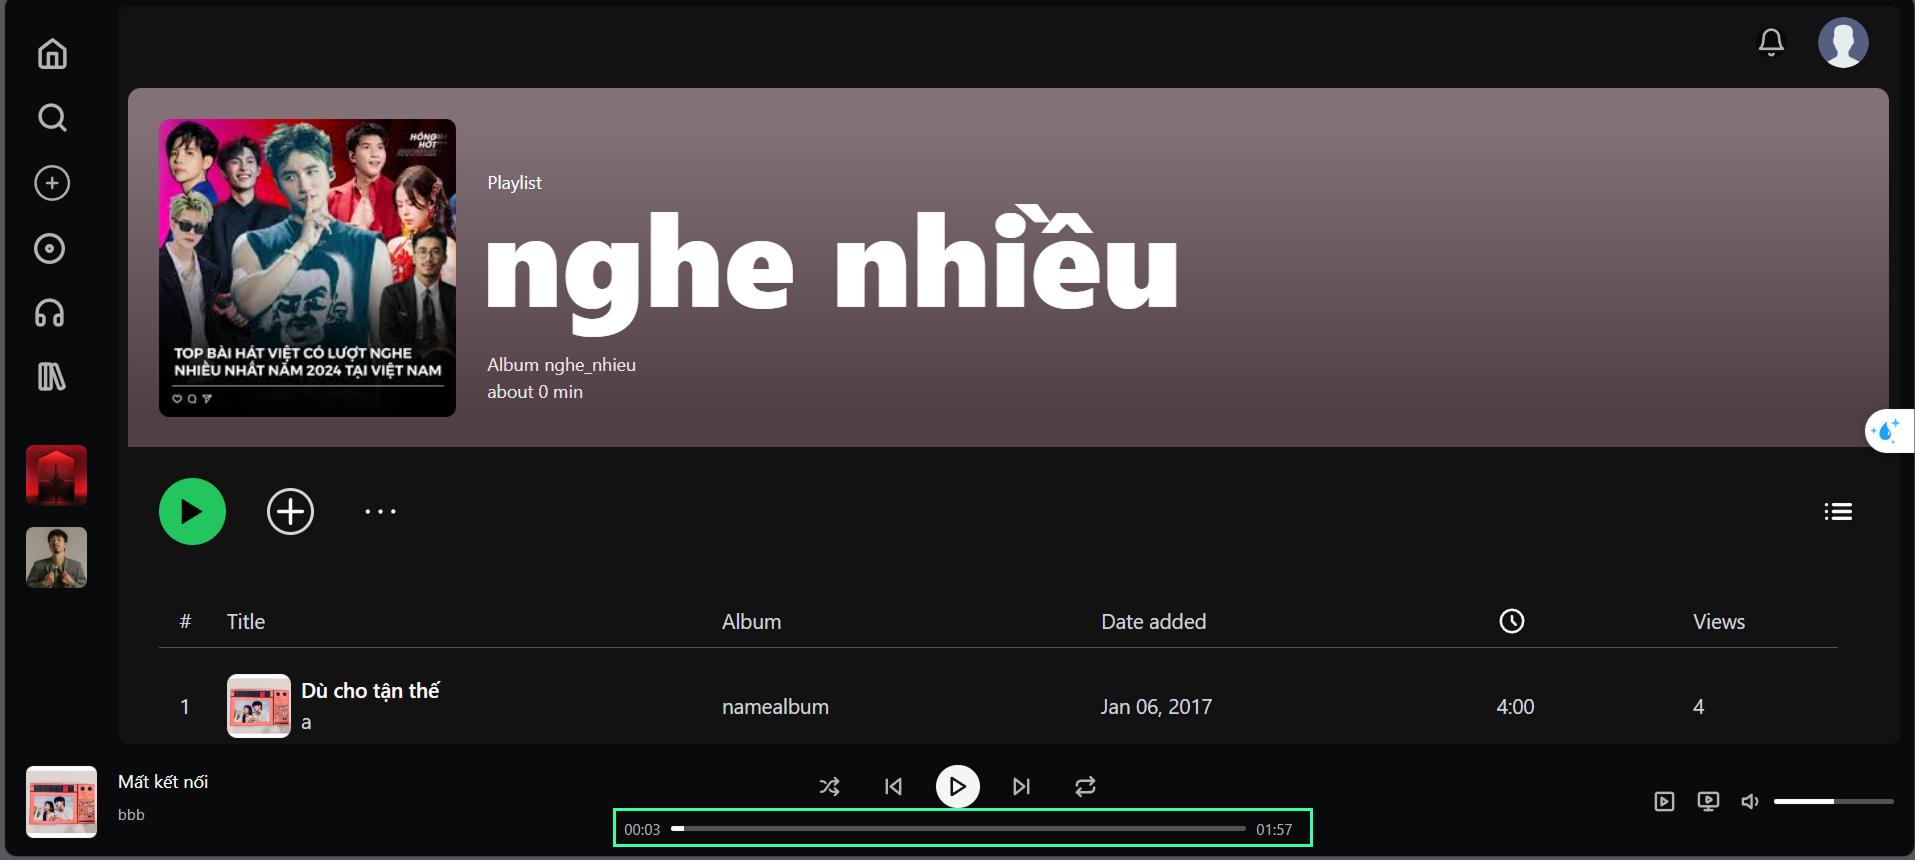
\includegraphics[width=0.9\textwidth]{imgs/trienkhaife/slider.png}
  \caption{Giao diện thanh tua tiến trình bài hát}
  \subsection*{Code minh họa: Luồng xử lý thanh tiến trình ControllerSlider}

\begin{itemize}
  \item \textbf{A. Nhận props và khởi tạo state:}
\begin{verbatim}
const [isDragging, setIsDragging] = useState(false);
const [currentTime, setCurrentTime] = useState([0]);
const sliderRef = useRef<HTMLSpanElement>(null);
const audio = document.querySelector('#audio-player');
\end{verbatim}

  \item \textbf{B. Lấy dữ liệu bài hát hiện tại và thời lượng:}
\begin{verbatim}
const { currentSong } = useSelector((state: RootState) => state.player);
const duration = audio?.duration ?? 0;
\end{verbatim}

  \item \textbf{C. Hàm xử lý tua khi người dùng thả chuột:}
\begin{verbatim}
const onSliderCommit = useCallback((value) => {
  if (audio && value[0] != null) {
    audio.currentTime = value[0];
    setCurrentTime(value);
  }
}, [audio]);
\end{verbatim}

  \item \textbf{D. Đồng bộ thời gian với audio mỗi 500ms:}
\begin{verbatim}
useEffect(() => {
  if (!audio || isDragging) return;
  const interval = setInterval(() => {
    setCurrentTime([audio.currentTime]);
  }, 500);
  return () => clearInterval(interval);
}, [isDragging, audio]);
\end{verbatim}

  \item \textbf{E. Giao diện thanh trượt:}
\begin{verbatim}
<Slider
  ref={sliderRef}
  value={currentTime}
  max={duration}
  min={0}
  step={1}
  disabled={currentSong?.the_loai === 'Advertisement'}
  onValueChange={(val) => setCurrentTime(val)}
  onValueCommit={(val) => onSliderCommit(val)}
  onPointerDown={() => setIsDragging(true)}
  onPointerUp={() => setIsDragging(false)}
/>
\end{verbatim}
\end{itemize}

\end{figure}

\vspace{1cm}

\section{VolumeController}

\textbf{Mục đích:} \textit{VolumeController} là thành phần điều khiển âm lượng, cho phép người dùng:
\begin{itemize}
  \item Tăng/giảm âm lượng nhạc đang phát.
  \item Bật hoặc tắt tiếng (mute).
  \item Thay đổi biểu tượng loa theo mức âm lượng.
\end{itemize}

\textbf{Luồng hoạt động:}
\begin{enumerate}
  \item \textbf{Khởi tạo:}
  \begin{itemize}
    \item Mặc định \texttt{volume = 0.5}.
    \item Gán \texttt{audioPlayer.volume = 0.5}.
  \end{itemize}

  \item \textbf{Kéo thanh âm lượng (Slider):}
  \begin{itemize}
    \item Cập nhật giá trị \texttt{volume = value[0] / 100}.
    \item Nếu \texttt{volume = 0} → tự động chuyển biểu tượng sang mute.
  \end{itemize}

  \item \textbf{Click biểu tượng loa (onMuteClick):}
  \begin{itemize}
    \item Toggle trạng thái \texttt{isMuted}.
    \item Gán lại \texttt{audioPlayer.muted = true/false}.
  \end{itemize}

  \item \textbf{Tự động chọn biểu tượng phù hợp:}
  \begin{itemize}
    \item \texttt{VolumeXIcon} nếu đang mute hoặc \texttt{volume = 0}.
    \item \texttt{VolumeIcon} nếu \texttt{volume < 0.3}.
    \item \texttt{Volume1Icon} nếu \texttt{volume < 0.6}.
    \item \texttt{Volume2Icon} nếu \texttt{volume $\geq$ 0.6}.
  \end{itemize}
\begin{figure}[H]
    \centering
    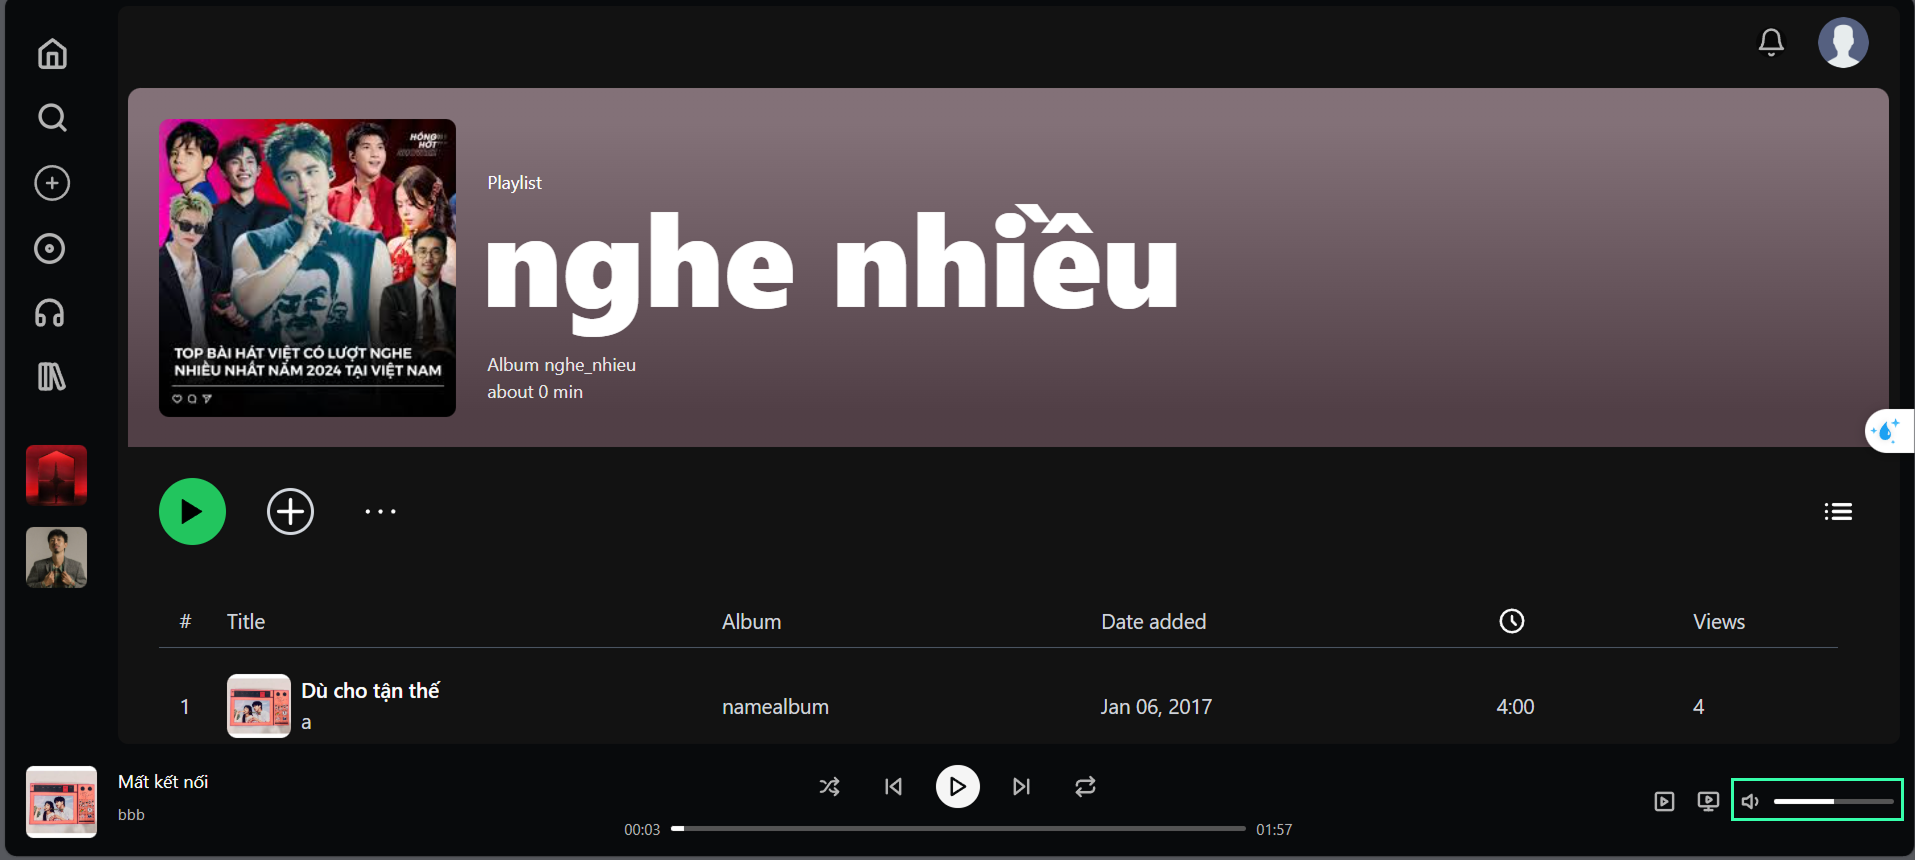
\includegraphics[width=0.6\textwidth]{imgs/trienkhaife/volume.png}
    \caption{Thanh điều chỉnh âm lượng và biểu tượng loa}
  \end{figure}
  \subsection*{Code minh hoạ luồng xử lý điều chỉnh âm lượng}

\begin{itemize}
  \item \textbf{A. Khởi tạo:}
  \begin{verbatim}
const [volume, setVolume] = useState(0.5)
const [isMuted, setIsMuted] = useState(false)
const audio = document.querySelector('#audio-player')
  \end{verbatim}

  \item \textbf{B. Khi kéo thanh âm lượng (Slider):}
  \begin{verbatim}
const onChange = (value) => {
  const vol = value[0] / 100
  setVolume(vol)
  audio.volume = vol
  setIsMuted(vol === 0)
}
  \end{verbatim}

  \item \textbf{C. Khi nhấn icon loa (mute/unmute):}
  \begin{verbatim}
const onMuteClick = () => {
  setIsMuted(!isMuted)
  audio.muted = !isMuted
}
  \end{verbatim}

  \item \textbf{D. Tự chọn icon phù hợp:}
  \begin{verbatim}
const Icon = isMuted || volume === 0
  ? VolumeXIcon
  : volume < 0.3 ? VolumeIcon
  : volume < 0.6 ? Volume1Icon
  : Volume2Icon
  \end{verbatim}

  \item \textbf{E. Giao diện:}
  \begin{verbatim}
<ControlButton Icon={Icon} onClick={onMuteClick} />
<Slider value={[volume * 100]} onValueChange={onChange} />
  \end{verbatim}
\end{itemize}

\end{enumerate}
